\hypertarget{ux5f15ux8a00}{%
\part{引言}\label{ux5f15ux8a00}}

\hypertarget{ux673aux5668ux5b66ux4e60ux4e3aux4ec0ux4e48ux9700ux8981ux7b56ux7565}{%
\chapter{机器学习为什么需要策略}\label{ux673aux5668ux5b66ux4e60ux4e3aux4ec0ux4e48ux9700ux8981ux7b56ux7565}}

\textbf{机器学习(machine
learning)}已然成为无数重要应用的基石------如今,在网络搜索、垃圾邮件检测、语音识别以及产品推荐等领域,你都能够发现它的身影。如果你或你的团队正在研发一款机器学习相关应用,并期待取得较快进展,那么这本书将会是你的得力助手。

案例:建立猫咪图片初创公司

想象一下,你正在建立一家初创公司,这家公司的产品目标是为猫咪爱好者们提供数不尽的猫咪图片,你打算应用\textbf{神经网络(neural
network)}技术来构建一套计算机视觉系统,通过该系统来识别图片中的猫。

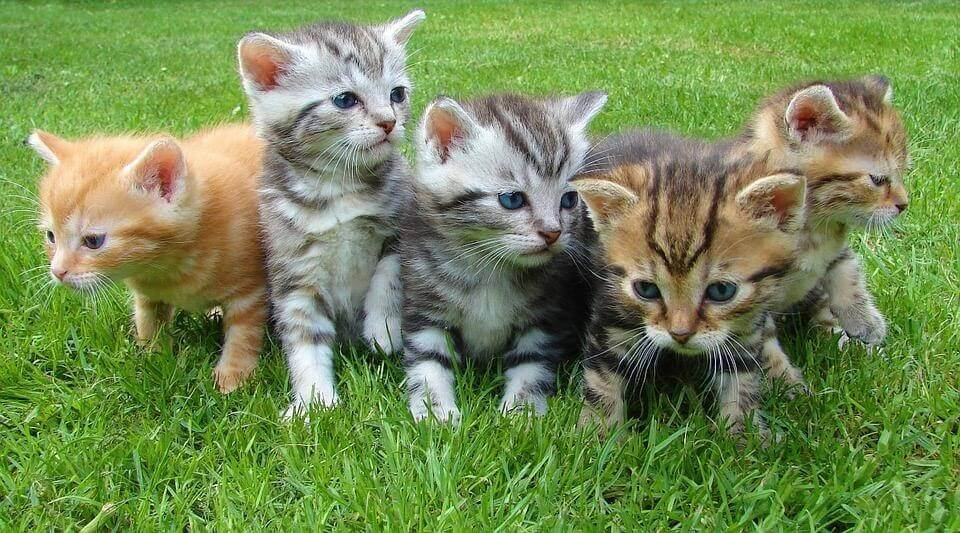
\includegraphics{./img/ch01_cats.jpg}

但悲剧的是,目前你的学习算法准确度还不够好。为了改进这个猫咪检测器,你正面临着巨大的压力。可你该怎么做呢?

你的团队给出了许多建议,例如:

\begin{itemize}
\tightlist
\item
  获取更多的数据,即收集更多的猫咪图片
\item
  收集更加多样化的训练数据集,图片中猫的位置可能不常见,也有可能颜色奇异,或者拍摄时使用不同的相机参数
\item
  通过增加梯度下降的迭代次数,使算法训练得久一些
\item
  尝试一个拥有更多层/更多隐藏元/更多参数的,规模更大的神经网络
\item
  尝试一个更小的神经网络
\item
  尝试加入正则化(例如 L2 正则化)
\item
  改变神经网络的架构(激活函数,隐藏元数量等等)
\item
  \ldots{}
\end{itemize}

在上面众多的方向中,如果你做出了正确的选择,就将建立起一个效果领先的猫咪图片识别平台,并带领你的公司取得成功。但如果你选择了一个糟糕的方向,则可能因此浪费掉几个月的时间。那么你该如何做出决定呢?

这本书将告诉你应该怎么做。众多的机器学习问题会留下一些线索,告诉你什么样的尝试有用,什么样的没用。而学会解读这些线索将会节省你几个月甚至几年的开发时间。

\hypertarget{ux5982ux4f55ux4f7fux7528ux6b64ux4e66ux6765ux5e2eux52a9ux4f60ux7684ux56e2ux961f}{%
\chapter{如何使用此书来帮助你的团队}\label{ux5982ux4f55ux4f7fux7528ux6b64ux4e66ux6765ux5e2eux52a9ux4f60ux7684ux56e2ux961f}}

完成本书的阅读后,你将进一步理解如何为一个机器学习项目设定技术方向,但团队成员可能不理解你为何要推荐某个特定的方向。有时你希望你的团队定义一个单值评估指标,但他们并不认可你的想法,此时你将如何说服他们?

这正是我决定缩短章节篇幅的原因------这样你就能够将它们打印出来,并且让你的成员仅阅读其中他们需要了解的那几页。

优先级的稍加改变会对团队的生产力产生巨大的影响,我希望你能帮助团队做出一些这样的改变,从而成为团队里的超级英雄!

\hypertarget{ux5148ux4feeux77e5ux8bc6ux4e0eux7b26ux53f7ux8bf4ux660e}{%
\chapter{先修知识与符号说明}\label{ux5148ux4feeux77e5ux8bc6ux4e0eux7b26ux53f7ux8bf4ux660e}}

如果你有学习过机器学习相关课程(例如我在 Coursera 开设的机器学习
MOOC),或者有过监督学习的应用经验,这本书的内容对你而言则不难理解。

本书假设你熟悉\textbf{监督学习(supervised
learning)}概念,即使用标注(labeled)的训练样本\((x,y)\)来学习一个从\(x\)映射到\(y\)的函数。监督学习算法主要包括线性回归(linear
regression)、对数几率回归(logistic
regression,又译作逻辑回归、逻辑斯蒂回归)和神经网络(neural
network)。虽然机器学习的形式有许多种,但当前具备实用价值的大部分机器学习算法都来自于监督学习。

我将经常提及神经网络(也被人们称为``深度学习''
),但你只需对这个概念有基础的了解便可以阅读本书后面的内容。

如果对上文提到的一些概念你还不是很熟悉,可以在 Coursera
观看《机器学习》前三周的课程内容。(课程地址:http://ml-class.org)

\hypertarget{ux89c4ux6a21ux9a71ux52a8ux673aux5668ux5b66ux4e60ux53d1ux5c55}{%
\chapter{规模驱动机器学习发展}\label{ux89c4ux6a21ux9a71ux52a8ux673aux5668ux5b66ux4e60ux53d1ux5c55}}

关于深度学习(神经网络)的一些想法在几十年前就有了,那为什么它们到现在才流行起来了呢?

推动其近期发展的主要因素有两个:

\begin{itemize}
\tightlist
\item
  \textbf{数据可用性(data
  availability)}:如今人们在数字设备(笔记本电脑、移动设备等)上花费的时间越来越多,对应的数字化行为与活动产生了海量的数据,而这些数据都可以提供给我们的学习算法用来训练。
\item
  \textbf{计算规模(computational
  scale)}:在近几年前,我们才开始有能力训练出规模足够大的神经网络来使用现有的海量数据集。
\end{itemize}

具体来说,即使你积累了更多的数据,但应用在类似于对数几率回归(logistic
regression)这样较传统的学习算法上,其性能表现(performance)也将趋于
``平稳'' 。这意味着算法的学习曲线将 ``变得平缓''
,就算提供更多的数据,算法的性能也将不再提升。

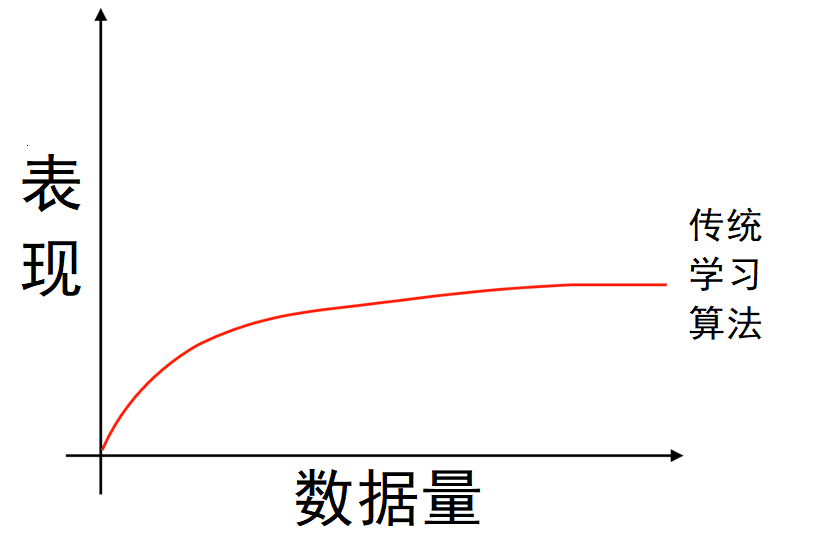
\includegraphics{./img/ch04_01.png}

传统学习算法似乎并不知道要如何来处理现今这般规模量级的数据。

在同样的监督学习任务下,选择训练一个小型的神经网络(neutral network,
NN),你可能会获得较好的性能表现:

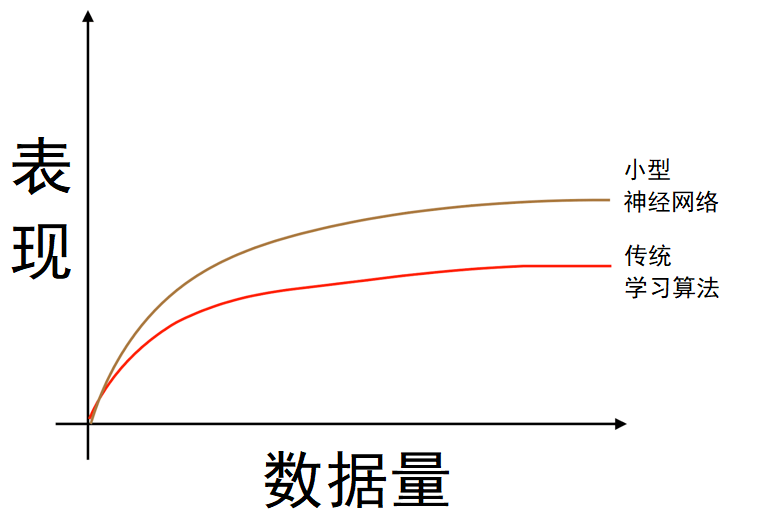
\includegraphics{./img/ch04_02.png}

\begin{quote}
该图显示了在小数据集上应用神经网络的效果会更好,但这种效果与将神经网络应用在大数据集时不太一致。在小数据集情况下,传统算法是否会表现得更好,取决于人们如何进行特征选择工程。例如,假设你只有
20
个训练样本,那么使用对数几率回归还是神经网络可能无关紧要;此时人为的特征选择工程比起选择哪种算法将产生更大的影响。但如果你有
100 万个样本数据,我会赞成你使用神经网络。
\end{quote}

这里的 ``小型神经网络''
指的是只含有少量的隐藏元/层/参数的神经网络。但如果你训练的神经网络规模越来越大,最终很有可能会获得更好的表现:

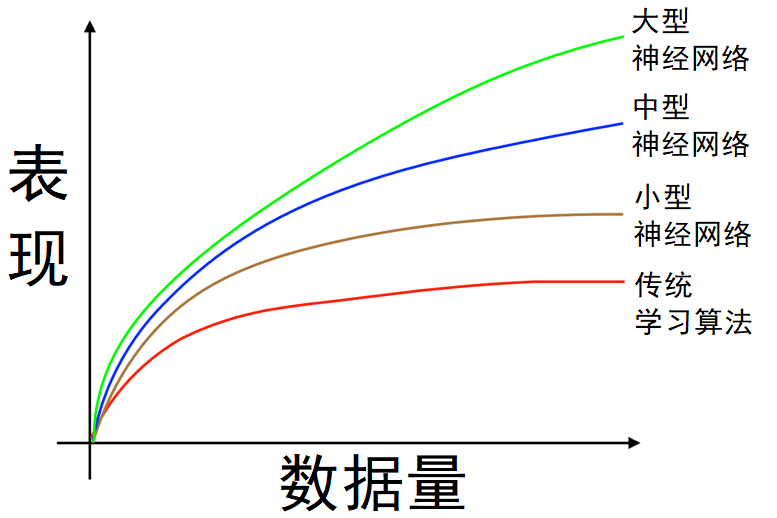
\includegraphics{./img/ch04_03.png}

因此,为了获得最佳的性能表现,你可以这样做:

\begin{enumerate}
\def\labelenumi{\arabic{enumi}.}
\item
  训练大型的神经网络,效果如同上图的绿色曲线;
\item
  拥有海量的数据。
\end{enumerate}

在算法训练时,许多其它的细节也同等重要,例如神经网络的架构。但目前来说,提升算法性能的更加可靠的方法仍然是训练更大的网络以及获取更多的数据。完成
1 和 2
的过程异常复杂,本书将对其中的细节作进一步的讨论。我们将从传统学习算法与神经网络中都起作用的通用策略入手,循序渐进地讲解至最前沿的构建深度学习系统的策略。

\hypertarget{ux8bbeux7f6eux5f00ux53d1ux96c6ux4e0eux6d4bux8bd5ux96c6}{%
\part{设置开发集与测试集}\label{ux8bbeux7f6eux5f00ux53d1ux96c6ux4e0eux6d4bux8bd5ux96c6}}

\hypertarget{ux5f00ux53d1ux96c6ux548cux6d4bux8bd5ux96c6ux7684ux5b9aux4e49}{%
\chapter{开发集和测试集的定义}\label{ux5f00ux53d1ux96c6ux548cux6d4bux8bd5ux96c6ux7684ux5b9aux4e49}}

继续分析我们之前提到的猫咪图片的案例:现在你负责运营一个移动端
app,用户会向这个 app 上传许多不同内容的图片。而你希望这个 app
能够从图片中自动地找到含有猫的图片。

你的团队已经在不同的网站下载了含有猫的图片(正样本,又译作正例),以及不含猫的图片(负样本,又译作反例),从而得到了一个巨型的数据集。他们将数据集按照
70\% / 30\% 的比例划分为训练集(training set)和测试集(test
set),并且使用这些数据构建出了一个在训练集和测试集上均表现良好的猫咪检测器。

可当你将这个分类器(classifier)部署到移动应用中时,却发现它的性能相当之差!

这究竟是什么原因导致的呢?

你会发现,从网站上下载下来作为训练集的图片与用户上传的图片有较大的区别------用户上传的图片大部分是使用手机拍摄的,此类图片往往分辨率较低,且模糊不清,采光也不够理想。但由于用来进行训练和测试的数据集图片均取自网站,这就导致了算法不能够很好地泛化(generalize)到我们所关心的手机图片的实际分布(actual
distribution)情况上。

在大数据时代来临前,机器学习中的普遍做法是使用 70\% / 30\%
的比例来随机划分出训练集和测试集。这种做法的确可行,但在越来越多的实际应用中,训练数据集的分布(例如上述案例中的网站图片)与人们最终所关心的分布情况(例如上述案例中的手机图片)往往不同,此时执意采取这样的划分其实是一个坏主意。

我们通常认为:

\begin{itemize}
\item
  \textbf{训练集(training set)}用于运行你的学习算法。
\item
  \textbf{开发集(development
  set)}用于调整参数,选择特征,以及对学习算法作出其它决定。有时也称为\textbf{留出交叉验证集(hold-out
  cross validation set)}。
\item
  \textbf{测试集(test
  set)}用于评估算法的性能,但不会据此改变学习算法或参数。
\end{itemize}

在定义了开发集(development set)和测试集(test
set)后,你的团队将可以尝试许多的想法,比如调整学习算法的参数来探索哪些参数的使用效果最好。开发集和测试集能够帮助你的团队快速检测算法性能。

换而言之,\textbf{开发集和测试集的使命就是引导你的团队对机器学习系统做出最重要的改变。}

所以你应当这样处理:

\begin{quote}
合理地选择开发集和测试集,使之能够代表将来实际数据的情况,并期望算法能够运行良好。
\end{quote}

也就是说你的测试集不应该仅是简单地将可用的数据划分出
30\%,尤其是将来获取的数据(移动端图片)在性质上可能会与训练集(网站图片)有所不同时。

如果你尚未推出移动端
app,那么可能还没有任何的用户,因此也无法获取一些准确的反馈数据来为后续的行动提供依据。但你仍然能够尝试去模拟出这种情况,例如邀请你的朋友用手机拍下照片并发送给你。当你的
app 上线后,就能够使用实际的用户数据对开发集和测试集进行更新。

如果你实在没有途径获取近似未来实际情况的数据,也可以尝试使用已有的网站图片。但你应该意识到这其中的风险,它将导致系统不能够很好地泛化(generalize)。

选择一个理想的开发集和测试集是需要一定投入的,投入多少由你来决定。但请不要武断地认为测试集分布和训练集分布是一致的。尽可能地选择你最终期望算法能够正确处理的样本作为测试集,而不是随便选择一个你恰好拥有的训练集样本。

\hypertarget{ux5f00ux53d1ux96c6ux548cux6d4bux8bd5ux96c6ux5e94ux8be5ux670dux4eceux540cux4e00ux5206ux5e03}{%
\chapter{开发集和测试集应该服从同一分布}\label{ux5f00ux53d1ux96c6ux548cux6d4bux8bd5ux96c6ux5e94ux8be5ux670dux4eceux540cux4e00ux5206ux5e03}}

根据公司的核心市场分布情况,你将猫咪 app 的图像数据划分为 ``美国'' 、
``中国'' 、 ``印度'' 和 ``其它地区''
四个区域。在设立开发集和测试集时,可以尝试将 ``美国'' 和 ``印度''
的数据归于开发集,而 ``中国'' 和 ``其它地区''
的数据归于测试集。也就是说我们可以随机地将其中两个区域的数据分配给开发集,另外两个区域的数据分配给测试集。\textbf{这样做对吗?}

当然不对!

一旦定义好了开发集和测试集,你的团队将专注于提升开发集的性能表现,这就要求开发集能够体现核心任务:使算法在四个地区都表现优异,而不仅仅是其中的两个。

开发集和测试集的分布不同还将导致第二个问题:你的团队所开发的系统可能在开发集上表现良好,却在测试集上表现不佳。我曾目睹过这样的事件,这令人十分沮丧并且还会浪费大量的时间,因此希望你不要重蹈他们的覆辙。

举个例子,假设你的团队开发了一套能在开发集上运行性能良好,却在测试集上效果不佳的系统。如果此时开发集和测试集的分布相同,那么你就能清楚地明白问题所在:算法在开发集上过拟合了(overfit)。解决方案显然就是去获取更多的开发集数据。

但是如果开发集和测试集服从不同的分布,解决方案就不那么明确了。此时可能存在以下一种或者多种情况:

\begin{enumerate}
\def\labelenumi{\arabic{enumi}.}
\tightlist
\item
  算法在开发集上过拟合了。
\item
  测试集比开发集更难进行预测,尽管算法做得足够好了,却很难有进一步的提升空间。
\item
  测试集不一定更难预测,但它与开发集性质并不相同(分布不同)。因此在开发集上表现良好的算法不一定在测试集上也能够取得出色表现。如果是这种情况,大量针对开发集性能的改进工作将会是徒劳的。
\end{enumerate}

构建机器学习应用已并非易事,而开发集和测试集分布的不匹配又会引入额外的不确定性------即提高算法在开发集上的性能表现,是否也能提升其在测试集的性能表现?在这种情况下很难去弄清楚哪些工作是有效的,哪些工作又是在浪费时间,从而会影响到工作的优先级安排。

在处理第三方基准测试(benchmark)问题时,样本提供方很可能已经指定了服从不同分布的开发集和测试集数据。与数据分布一致的情况相比,此时运气带来的性能影响将超过你使用的技术所带来的影响。因此,寻找能够在某个分布上进行训练,同时也能够很好地泛化到另一个分布上的学习算法,同样是一个重要的研究课题。但是如果你想要在特定的机器学习应用上取得进展,而不是搞研究,我建议你尽可能地选择服从相同分布的开发集和测试集数据,这会让你的团队更有效率。

\hypertarget{ux5f00ux53d1ux96c6ux548cux6d4bux8bd5ux96c6ux5e94ux8be5ux6709ux591aux5927}{%
\chapter{开发集和测试集应该有多大?}\label{ux5f00ux53d1ux96c6ux548cux6d4bux8bd5ux96c6ux5e94ux8be5ux6709ux591aux5927}}

开发集的规模应该尽可能的大,至少要能够区分出你所尝试的不同算法之间的性能差异。例如,如果分类器
A 的准确率为 90.0\% ,而分类器 B 的准确率为 90.1\% ,那么使用仅含有 100
个样本的开发集将无法检测出这 0.1\%
的差异。与我所遇到的机器学习问题相比,一个样本容量仅为 100
的开发集,规模太小了。通常来说,开发集的规模应该在 1,000 到 10,000
个样本数据之间,而当开发集样本容量为 10,000 时,你将很有可能检测到这
0.1\% 的性能提升。

\begin{quote}
从理论上来说,我们还可以检测算法的变化是否对开发集存在统计学意义上的显著差异。
然而在实践中,大多数团队并不会执着于此(除非他们正在发表学术研究论文),而且,通常在检测过程中,我并没有发现统计显著性检验能够起到多少作用。
\end{quote}

在类似广告服务、网络搜索和产品推荐等较为成熟且关键的应用领域,我曾见过一些团队非常积极地去改进算法性能,哪怕只有
0.01\%
的提升,因为这将直接影响到公司的利润。在这种情况下,开发集规模可能远超过
10,000 个样本,从而有利于检测到那些不易察觉的效果提升。

那么测试集的大小又该如何确定呢?它的规模应该大到使你能够对整体系统的性能进行一个高度可信的评估。一种常见的启发式策略是将整体
30\% 的数据用作测试集,这适用于总体数据量规模一般的情况(比如 100 至
10,000
个样本)。但是在大数据时代,有时我们所面临的机器学习问题的样本数量将超过
10
个亿,即使开发集和测试集中样本的绝对数量一直在增长,可总体上分配给开发集和测试集的数据比例正在不断降低。可以看出,我们并不需要将开发集和测试集的规模提升到远远超过评估算法性能所需的程度,也就是说,开发集和测试集的规模并不是越大越好。

\hypertarget{ux4f7fux7528ux5355ux503cux8bc4ux4f30ux6307ux6807ux8fdbux884cux4f18ux5316}{%
\chapter{使用单值评估指标进行优化}\label{ux4f7fux7528ux5355ux503cux8bc4ux4f30ux6307ux6807ux8fdbux884cux4f18ux5316}}

所谓的\textbf{单值评估指标(single-number evaluation
metric)}有很多,分类准确率就是其中的一种:待你在开发集(或测试集)上运行分类器之后,它将返回单个数值,代表着样本被正确分类的比例。根据这个指标,如果分类器
A 的准确率为 97%,而分类器 B 的准确率为 90\%,那么我们可以认为分类器 A
更优秀。

相比之下,\textbf{查准率}(Precision,又译作精度)和\textbf{查全率}(Recall,又译作召回率)的组合并不能作为单值评估指标,因为它给出了两个值来对你的分类器进行评估。多值评估指标提高了在算法之间进行优劣比较的难度,假设你的算法表现如下:

\begin{longtable}[]{@{}lll@{}}
\toprule
Classifier & Precision & Recall \\
\midrule
\endhead
A & 95\% & 90\% \\
B & 98\% & 85\% \\
\bottomrule
\end{longtable}

\begin{quote}
猫分类器的查准率指的是在开发集(或测试集)内,那些已经被预测为``猫''的图片之中,实际类别是``猫''的样本比例。而查全率指的是在开发集(或测试集)内,所有实际类别为``猫''的图片中,被正确预测为``猫''的样本比例。人们常常在查准率和查全率之间权衡取舍。
\end{quote}

若根据上方表格中的数值对两个分类器进行比较,显然二者都没有较为明显的优势,因此也无法指导你立即做出选择。

\begin{longtable}[]{@{}llll@{}}
\toprule
Classifier & Precision & Recall & F1 score \\
\midrule
\endhead
A & 95\% & 90\% & \textbf{92.4\%} \\
\bottomrule
\end{longtable}

当你的团队在进行开发时,往往会尝试多种多样的算法架构、模型参数、特征选择,或是一些其它的想法。你可以通过使用单值评估指标(如准确率),根据所有的模型在此指标上的表现,进行排序,从而能够快速确定哪一个模型的性能表现最好。

如果你认为查准率和查全率指标很关键,可以参照其他人的做法,将这两个值合并为一个值来表示。例如取二者的平均值,或者你可以计算
``F1分数(F1 score)''
,这是一种经过修正的平均值计算方法,比起直接取平均值的效果会好一些。

\begin{longtable}[]{@{}llll@{}}
\toprule
Classifier & Precision & Recall & F1 score \\
\midrule
\endhead
A & 95\% & 90\% & \textbf{92.4\%} \\
B & 98\% & 85\% & \textbf{91.0\%} \\
\bottomrule
\end{longtable}

\begin{quote}
如果你想了解更多关于 F1 分数的信息,可以参考
\url{https://en.wikipedia.org/wiki/F1_score}
它是查准率和查全率的调和平均数,计算公式为 2 / ( (1/Precision) +
(1/Recall) ).
\end{quote}

综上可知,当你需要在多个分类器之间进行选择时,使用单值评估指标将帮助你更快速地作出决定。它能给出一个清晰明了的分类器性能排名,从而帮助团队明确后续的改进方向。

最后补充一个例子,假设你在 ``美国'' 、 ``印度'' 、 ``中国'' 和
``其它地区''
这四个关键市场追踪你的猫分类器准确率,并且获得了四个指标。通过对这四个指标取平均值或进行加权平均,你将得到一个单值指标。\textbf{取平均值或者加权平均值是将多个指标合并为一个指标的最常用方法之一。}

\hypertarget{ux4f18ux5316ux6307ux6807ux548cux6ee1ux610fux5ea6ux6307ux6807}{%
\chapter{优化指标和满意度指标}\label{ux4f18ux5316ux6307ux6807ux548cux6ee1ux610fux5ea6ux6307ux6807}}

下面我们来了解一下组合多个评估指标的另一种方法。

假设你既关心学习算法的准确率(accuracy),又在意其运行时间(running
time),请从下面的三个分类器中做出选择:

\begin{longtable}[]{@{}lll@{}}
\toprule
Classifier & Accuracy & Running time \\
\midrule
\endhead
A & 90\% & 80ms \\
B & 92\% & 95ms \\
C & 95\% & 1,500ms \\
\bottomrule
\end{longtable}

将准确率和与运行时间放入单个公式计算后可以导出单个的指标,这似乎不太符合常理,例如:

\[
Accuracy - 0.5 * RunningTime
\]

有一种替代方案可供选择:首先定义一个 ``可接受的'' 运行时间,一般低于
100ms
。接着,在限定的运行时间范围内,尽可能地将分类器的准确率最大化。此时,运行时间代表着
``满意度指标'' ------ 你的分类器必须在这个指标上表现得 ``足够好''
,这里指的是运行时间约束上限为 100ms;而准确度则代表着 ``优化指标''。

如果要考虑\(N\)项不同的标准,比如模型的二进制文件大小(这对移动端 app
尤为重要,因为用户不想下载体积很大的
app)、运行时间和准确率,你或许需要设置\(N-1\)个 ``满意度''
指标,即先要求它们满足一定的值或范围,下一步才是定义一个 ``优化''
指标。例如分别为二进制文件的大小和运行时间设定可接受的阈值,并尝试根据这些限制来优化准确率指标。

最后再举一个例子,假设你正在设计一个硬件设备,该设备可以根据用户设置的特殊
``唤醒词'' 来唤醒系统,类似于 Amazon Echo 的监听词为
``Alexa'',苹果(Apple) Siri 的监听词为 ``Hey Siri'',安卓(Android)
的监听词为 ``Okay Google'',以及百度(Baidu)应用的监听词 ``Hello
Baidu.'' 我们关心的指标是假正例率(false positive
rate,又译作假阳率,误诊率)------
用户没有说出唤醒词,系统却被唤醒了,以及假反例率(false negative
rate,又译作假阴率,漏诊率)------用户说出了唤醒词,系统却没能正确被唤醒。这个系统的一个较为合理的优化对象是尝试去最小化假反例率(优化指标),减少用户说出唤醒词而系统却没能正确唤醒的发生率,同时设置约束为每
24 小时不超过一次误报(满意度指标)。

一旦你的团队在优化评估指标上保持一致,他们将能够取得更快的进展。

\hypertarget{ux901aux8fc7ux5f00ux53d1ux96c6ux548cux5ea6ux91cfux6307ux6807ux52a0ux901fux8fedux4ee3}{%
\chapter{通过开发集和度量指标加速迭代}\label{ux901aux8fc7ux5f00ux53d1ux96c6ux548cux5ea6ux91cfux6307ux6807ux52a0ux901fux8fedux4ee3}}

对于当前面临的新问题,我们很难提前知道使用哪种方法会是最合适的,即使是一个经验丰富的机器学习研究员,通常也需要在尝试多种多样的方法之后才能发现令人满意的方案。当我要建立一个机器学习系统时,往往会这么做:

\begin{enumerate}
\def\labelenumi{\arabic{enumi}.}
\tightlist
\item
  尝试一些关于系统构建的\textbf{想法(idea)}。
\item
  使用\textbf{代码(code)}实现想法。
\item
  根据\textbf{实验(experiment)}结果判断想法是否行得通。(第一个想到的点子一般都行不通!)在此基础上学习总结,从而产生新的想法,并保持这一迭代过程。迭代过程如下图所示:
\end{enumerate}

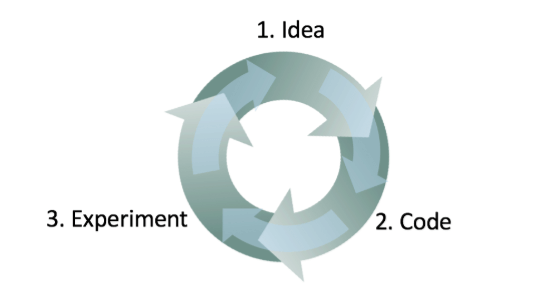
\includegraphics{./img/ch10_01.png}

迭代过程循环得越快,你也将进展得越快。此时,拥有开发集、测试集和度量指标的重要性便得以体现了:每当你有了一个新想法,在开发集上评估其性能就可以帮助你判断当前的方向是否正确。

假如你没有一个特定的开发集和度量指标,则需要在每次开发新的分类器时把它整合到
app
中,并通过几个小时的体验来了解分类器的性能是否有所改进------这会浪费大量的时间!另外,如果你的团队将分类器的准确率从
95.0% 提高到 95.1%,这 0.1\%
的提升可能很难被检测出来。但是积少成多,通过不断积累这 0.1%
的改进,你的系统将取得巨大的提升。拥有开发集和度量指标,可以使你更快地检测出哪些想法给系统带来了小(或大)的提升
,从而快速确定下一步要研究或者是要放弃的方向。

\hypertarget{ux4f55ux65f6ux4feeux6539ux5f00ux53d1ux96c6ux6d4bux8bd5ux96c6ux548cux6307ux6807}{%
\chapter{何时修改开发集、测试集和指标}\label{ux4f55ux65f6ux4feeux6539ux5f00ux53d1ux96c6ux6d4bux8bd5ux96c6ux548cux6307ux6807}}

每当开展一个新项目时,我会尽快选好开发集和测试集,因为这可以帮团队制定一个明确的目标。

我通常会要求我的团队在不到一周(一般不会更长)的时间内给出一个初始的开发集、测试集和指标,提出一个不太完美的方案并迅速执行
,这比起花过多的时间去思考要好很多。但是一周的时间要求并不适用于成熟的应用程序,譬如垃圾邮件过滤。我也见到过一些团队在已经成熟的系统上花费数月的时间来获得更好的开发集和测试集。

如果你渐渐发现初始的开发集、测试集和指标设置与期望目标有一定差距,那就尽快想办法去改进它们。例如你的开发集与指标在排序时将分类器
A 排在 B 的前面,然而你的团队认为分类器 B
在实际产品上的表现更加优异,这个时候就需要考虑修改开发集和测试集,或者是你的评估指标了。

在上述例子中,有三个主要原因可能导致开发集/评估指标错误地将分类器A排在B前面:

\begin{enumerate}
\def\labelenumi{\arabic{enumi}.}
\item
  \textbf{你需要处理的实际数据的分布和开发集/测试集数据的分布情况不同。}

  假设你的初始开发集和测试集中主要是成年猫的图片,然而你在 app
  上发现用户上传的更多是小猫的图片,这就导致了开发集和测试集的分布与你需要处理数据的实际分布情况不同。在这种情况下,需要更新你的开发集和测试集,使之更具代表性。
\item
  \textbf{算法在开发集上过拟合了。}

  在开发集上反复评估某个想法会导致算法在开发集上 ``过拟合''
  。当你完成开发后,应该在测试集上评估你的系统。如果你发现算法在开发集上的性能比测试集好得多,则表明你很有可能在开发集上过拟合了。在这种情况下,你需要获取一个新的开发集。

  如果需要跟踪团队的进度,你可以每周或者每月在测试集上对系统进行一次定期评估。但不要根据测试集指标对算法做出任何决策,包括是否将系统回滚到前一周的状态。坚持这样做会导致算法在测试集上开始过拟合,并且不要再指望通过测试集对你的系统性能进行完全无偏估计(这对发表研究论文以及需要做出商业决策的人来说影响很大)。
\item
  \textbf{该指标不是项目应当优化的目标。}

  假设你的猫咪 app 当前的指标为分类准确率,而该指标认为分类器 A
  优于分类器 B。然而在尝试了两种算法后,你发现分类器 A
  竟然允许出现一些色情图片,这实在是难以容忍。应该怎么办呢?

  以上这种情况表明,此时的指标并不能辨别出算法 B
  在实际产品中的表现是否比 A
  更好,因此根据该指标来选择算法并不可靠,也说明此时应该改变现有的评估指标。你可以选择修改指标,使之对出现色情图片的情况执行严重惩罚。此外,强烈建议你选择一个新的指标并为你的团队制定一个新的研究目标,而不是在不可信的指标上耗费太多的时间,最终导致不得不回过头对分类器进行人工选择。
\end{enumerate}

在项目中改变开发集、测试集或者指标是很常见的。一个初始的开发集、测试集和指标能够帮助团队进行快速迭代,当你发现它们对团队的导向不正确时,不要担心,你只需要对其进行修改并确保团队能够了解接下来的新方向。

\hypertarget{ux5c0fux7ed3ux5efaux7acbux5f00ux53d1ux96c6ux548cux6d4bux8bd5ux96c6}{%
\chapter{小结:建立开发集和测试集}\label{ux5c0fux7ed3ux5efaux7acbux5f00ux53d1ux96c6ux548cux6d4bux8bd5ux96c6}}

\begin{itemize}
\tightlist
\item
  被选择作为开发集和测试集的数据,应当与你未来计划获取并对其进行良好处理的数据有着相同的分布,而不一定和训练集的数据分布一致。
\item
  开发集和测试集的分布应当尽可能一致。
\item
  为你的团队选择一个单值评估指标进行优化。当需要考虑多项目标时,不妨将它们整合到一个表达式里(比如对多个误差指标取平均),或者设定满意度指标和优化指标。
\item
  机器学习是一个高度迭代的过程:在出现最终令人满意的方案之前,你可能要尝试很多想法。
\item
  拥有开发集、测试集和单值评估指标可以帮助你快速评估一个算法,从而加速迭代进程。
\item
  当你要探索一个全新的应用时,尽可能在一周内建立你的开发集、测试集和评估指标;而在已经相对成熟的应用上,可以考虑花费更长的时间来执行这些工作。
\item
  传统的 70\% / 30\%
  训练集/测试集划分对于大规模数据并不适用,实际上,开发集和测试集的比例会远低于
  30\%.
\item
  开发集的规模应当大到能够检测出算法精度的细微改变,但也不需要太大;测试集的规模应该大到能够使你能对系统的最终性作出一个充分的估计。
\item
  当开发集和评估指标对于团队已经不能提供一个正确的导向时,尽快修改它们:(i)
  如果算法在开发集上过拟合,则需要获取更多的开发集数据。(ii)
  如果开发集与测试集的数据分布和实际数据分布不同,则需要获取新的开发集和测试集。
  (iii) 如果评估指标无法对最重要的任务目标进行度量,则需要修改评估指标。
\end{itemize}

\hypertarget{ux57faux7840ux8befux5deeux5206ux6790}{%
\part{基础误差分析}\label{ux57faux7840ux8befux5deeux5206ux6790}}

\hypertarget{ux5febux901fux6784ux5efaux5e76ux8fedux4ee3ux4f60ux7684ux7b2cux4e00ux4e2aux7cfbux7edf}{%
\chapter{快速构建并迭代你的第一个系统}\label{ux5febux901fux6784ux5efaux5e76ux8fedux4ee3ux4f60ux7684ux7b2cux4e00ux4e2aux7cfbux7edf}}

当你想要构建一个新的垃圾邮件过滤系统时,团队可能会有各式各样不同的想法:

\begin{itemize}
\tightlist
\item
  收集海量的垃圾邮件作为训练集。例如,设置一个
  ``蜜罐(honeypot,计算机安全领域又称为诱饵)'',故意地向垃圾邮件系统发送一些虚假邮件地址,以便于能够自动收集到垃圾邮件系统发送到这些地址的垃圾邮件内容。
\item
  开发用于理解邮件文本内容的功能。
\item
  开发用于理解邮件信封或邮件头部特征的功能,据此了解邮件经由了哪些网络服务器进行中转。
\item
  更多\ldots{}
\end{itemize}

虽然我在反垃圾邮件领域已经有了一定的经验,却依然难以保证每次都能顺利在上面的方向中进行抉择。如果你在此领域并不是一个专家,难度会变得更大。

如果在一开始就试图设计和构建出完美的系统会显得有些困难,不妨先花几天时间构建并训练一个最基础的系统。

\begin{quote}
这个建议旨在帮助那些想要构建 AI
应用的读者,而不是那些想要发表研究论文的人,我将会在之后的内容中提到与研究有关的话题。
\end{quote}

或许这个最基础的系统与我们所能构建的 ``最佳''
系统相去甚远,但研究其中的基础功能也是很有价值的:你能快速找到一些线索来帮助你决定在什么方向上投入时间。后面的一些章节会向你剖析该如何解读这些线索。

\hypertarget{ux8befux5deeux5206ux6790ux6839ux636eux5f00ux53d1ux96c6ux6837ux672cux8bc4ux4f30ux60f3ux6cd5}{%
\chapter{误差分析:根据开发集样本评估想法}\label{ux8befux5deeux5206ux6790ux6839ux636eux5f00ux53d1ux96c6ux6837ux672cux8bc4ux4f30ux60f3ux6cd5}}

在使用猫咪 app
时,你注意到它将一些狗的图片误分类为猫了,因为有些狗的样子的确很像猫。

团队中有人建议,加入第三方软件来帮助系统更好地处理狗的样本,但这需要一个月的时间去完成。面对团队成员高涨的热情,你会允许他们这样做吗?

在执行这项计划前,我建议你先预估一下该任务能提升多少系统精度。这样你就能够更加理性地判断是否值得花一个月的时间做这件事,还是将这段时间用于其它任务。

具体而言,你可以这样:

\begin{enumerate}
\def\labelenumi{\arabic{enumi}.}
\tightlist
\item
  收集 100 个开发集中被误分类的样本,即造成系统误差的样本。
\item
  人为查看这些样本,并计算其中狗的比例。
\end{enumerate}

查看误分类样本的这一过程称为\textbf{误差分析}。在上面的例子中,如果只有
5\%
误分类的图像是狗,那么无论你在狗的问题上做多少的算法改进,最终都不会消除超过原有的
5\% 误差 . 也即是说 5\%
是该计划项目所能起到帮助的``上限''(最大可能值)。所以如果整个系统当前的精度为
90\%(对应误差为 10\%),那么这种改进最多能将精度提升到 90.5\%
(对应误差下降到 9.5\% , 改进了原有 10\% 误差其中的 5\%)。

相反,如果你发现 50\%
的误分类图像是狗,那就可以自信地说这个项目将效果明显,它可以将精度从
90\% 提升到 95\% (相对误差减少 50\%,整体误差由 10\% 下降到 5\%)。

这种简单的误差分析计算过程可以协助你快速评估,从而了解是否需要将处理狗样本的第三方软件进行整合。它为是否值得进行这项投入给出了一个量化的基准。

误差分析也可以帮助你在不同的想法中发现哪些想法将更有前景。我见过许多工程师不愿意进行误差分析,他们更倾向于直接提出一个并实现一个想法,而不考虑该想法是否值得花时间去投入。这是一个普遍的误解:后果可能是你的团队在耗费一个月的时间后却发现收益甚少。

人为检查 100
个样本并不会占用太多的时间。即使你每分钟只检查一张图片,也能够在两小时内完成,而这两个小时可能可以帮你节省一个月的工作量。

\textbf{误差分析}(Error Analysis)
指的是检查被算法误分类的开发集样本的过程,以便帮助你找到造成这些误差的原因。这将协助你确定各个项目的优先级(就像上面的例子所提到的那样)并且获得探索新方向的灵感,我们将会在之后再讨论这些内容。接下来的几章会给出一些误差分析的最佳实践。

\hypertarget{ux5728ux8befux5deeux5206ux6790ux65f6ux5e76ux884cux8bc4ux4f30ux591aux4e2aux60f3ux6cd5}{%
\chapter{在误差分析时并行评估多个想法}\label{ux5728ux8befux5deeux5206ux6790ux65f6ux5e76ux884cux8bc4ux4f30ux591aux4e2aux60f3ux6cd5}}

对于改进猫检测器,你的团队有一些想法:

\begin{itemize}
\tightlist
\item
  修正算法将狗误分类为猫的问题。
\item
  修正算法将大型猫科动物(比如狮子、黑豹等等,下面用大猫代指)误分类为家猫的问题。
\item
  改善系统在模糊图像上的表现。
\item
  \ldots{}
\end{itemize}

上述的想法都可以以并行的形式进行评估。通常我会创建一个电子表格,一边查看被误分类的
100
个开发集样本一边完善表格内容,同时我也会留下一些能够帮助我记住特定样本的备注。为了说明这一过程,如下所示是一个仅含四个样本的小型开发集的电子表格:

\begin{longtable}[]{@{}lllll@{}}
\toprule
图像 & 狗 & 大猫 & 模糊 & 备注 \\
\midrule
\endhead
1 & √ & & & 不常见的美国比特犬 \\
2 & & & √ & \\
3 & & √ & √ & 狮子;雨天在动物园拍摄的图片 \\
4 & & √ & & 树木后的美洲豹 \\
占全体比例 & 25\% & 50\% & 50\% & \\
\bottomrule
\end{longtable}

你会发现表格中图片 3
的''大猫''与``模糊''列都被勾选了,另外由于一个样本可能与多个类别都有关联,所以表格底部的百分比加起来可能不是
100 \%.

虽然你可能事先规定了一些类别(狗,大猫,模糊)并进行了手动的分类,但在浏览图像时你可能会受到启发并发现一些新的类别。比如你在浏览一些图片时发现,经过
Instagram
滤镜处理过的图片在识别时对结果造成了误差,你就可以在电子表格中加入一个新的
``Instagram''
列。手动查看误分类样本,并思考人类如何/是否能正确地分类这些样本,这将帮助你发现新的类别以及解决方案。

探寻方法去改进对应误差的类别是很有帮助的。举个例子,如果你能``撤销''
Instagram 的滤镜效果并恢复到原始图片,那么 Instagram
分类就能发挥作用。这不代表你只能局限于那些已有的改进途径的类别;这个过程主要是为了帮助你对一些潜在的,有改进效果的方向培养一定的敏感度。

假设你已检查了 100 个开发集的误分类样本,并得到了下面的表格:

\begin{longtable}[]{@{}lllll@{}}
\toprule
图像 & 狗 & 大猫 & 模糊 & 备注 \\
\midrule
\endhead
1 & √ & & & 不常见的美国比特犬 \\
2 & & & √ & \\
3 & & √ & √ & 狮子;雨天在动物园拍摄的图片 \\
4 & & √ & & 树木后的美洲豹 \\
\ldots{} & \ldots{} & \ldots{} & \ldots{} & \\
占全体比例 & 8\% & 43\% & 61\% & \\
\bottomrule
\end{longtable}

现在你应该可以判断出,对于解决狗的误分类问题项目最多可以改进 8\%
的误差,处理大猫和模糊类则可以改进更多。因此你将更有可能挑选后两者之一进行处理。如果你的团队有足够的人力并行处理多个方向,则可以要求一部分成员处理大猫类别,另一部分成员处理模糊类别。

误差分析并不会产生一个明确的数学公式来告诉你什么任务的优先级最高。你还需要考虑在不同类别上的预期进展以及解决每个类别所需的工作量。

\hypertarget{ux6e05ux6d17ux8befux6807ux6ce8ux7684ux5f00ux53d1ux96c6ux548cux6d4bux8bd5ux96c6ux6837ux672c}{%
\chapter{清洗误标注的开发集和测试集样本}\label{ux6e05ux6d17ux8befux6807ux6ce8ux7684ux5f00ux53d1ux96c6ux548cux6d4bux8bd5ux96c6ux6837ux672c}}

在进行误差分析时,你可能会注意到一些开发集的样本被误标注(mislabeled
)了。此处的``误标注''指的是图像在使用算法处理前,已经被负责标注的人员进行了错误的标注,也就是说,某个样本
\((x,y)\) 的分类标签(label)\(y\)
的值并不正确。例如,一些不是猫的图片被误标注为猫,反之亦然。如果你不确定这些被误标注的图片是否起着关键作用,可以添加一个类别来跟踪记录误标注样本的比例:

\begin{longtable}[]{@{}llllll@{}}
\toprule
图像 & 狗 & 大猫 & 模糊 & 误标注 & 备注 \\
\midrule
\endhead
\ldots{} & & & & & \\
89 & & & & √ & 标注者忽略了背景中的猫 \\
99 & & √ & & & \\
100 & & & & √ & 猫的画像;非真猫 \\
占全体比例 & 8\% & 43\% & 61\% & 6\% & \\
\bottomrule
\end{longtable}

那么这个时候,需要修正开发集中的标签吗?回忆一下当初设立开发集的目标------帮助你快速评估算法性能,从而判断算法
A 和 B
哪一个更好。如果开发集中误标注的部分的确影响了你的判断,那么花时间去修正这些标签就是值得的。

举个例子,假设你的分类器表现如下:

\begin{itemize}
\tightlist
\item
  开发集整体精度\ldots\ldots\ldots\ldots\ldots.. 90\% (10\% 整体误差)
\item
  误标注样本造成的误差\ldots\ldots{} 0.6\% (6\% 开发集误差)
\item
  其它原因造成的误差\ldots\ldots\ldots. 9.4\% (94\% 开发集误差)
\end{itemize}

相对于你正在改进的 9.4\% 误差,误标记的 0.6\%
误差看起来就不那么重要了。在开发集中手动修正误标注样本不会带来不好的影响,但这样的做法并不是必要的:当你不知道整个系统的误差是
10\% 还是 9.4\% 时,这样处理会看起来不错。

假设你不断地改进猫分类器,并达到了以下性能:

\begin{itemize}
\tightlist
\item
  开发集整体精度\ldots\ldots\ldots\ldots\ldots.. 98.0\% (2.0\%
  整体误差)
\item
  误标注样本造成的误差\ldots\ldots{} 0.6\% (30\% 开发集误差)
\item
  其它原因造成的误差\ldots\ldots\ldots. 1.4\% (70\% 开发集误差)
\end{itemize}

此时 30\%
的开发集误差是由误标注样本造成的,这对精度估计造成了显著的影响。此时就应该考虑改进开发集样本中的标签质量。处理这些误标注的样本将帮助你找出分类器的误差是接近
1.4\% 还是 2.0\% ,差异显著。

在项目初始阶段容许一些误标注的开发集/测试集样本并不罕见,你可以选择在系统改进到一定程度时再来考虑被误标注的样本,因为这些误差在整体误差中的占比会逐渐增大。

上一章中解释了如何通过算法改进类似于狗、大猫和模糊图片的误差类别,而在本章你学习了如何通过修正数据的标签来处理误标注的样本。

不论你使用什么方式修正开发集标签,请记住,要将同样的方式应用于你的测试集,这可以保持二者服从相同的分布。我们在第
6
章中已经讨论过了这样操作的意义,在那个问题中,团队成员花费了很多时间优化开发集,直到后来才意识到他们正在根据不同的测试集以不同的标准进行判断。

如果你决定改进标签质量,请仔细检查系统中被误分类和正确分类的样本的标签。对于某个样本,可能原始标注和算法预测的标签都是错误的。如果你仅修复系统误分类的样本标签,则有可能在评估中引入偏差。假设你有
1000 个开发集样本,同时分类准确率为 98\%,那么检查 20
个误分类的样本会比检查 980
个正确分类的样本要容易得多。由于在实际操作中,检查误分类样本较为容易,这就导致了开发集会衍生出一定的偏差。如果你只对开发产品和应用感兴趣,如此程度的偏差是可以接受的。但如果你计划在学术论文中引用此结果,可能就需要完全无偏地度量测试集的精度,此时这样做就会出现问题。

\hypertarget{ux5c06ux5927ux578bux5f00ux53d1ux96c6ux62c6ux5206ux4e3aux4e24ux4e2aux5b50ux96c6ux4e13ux6ce8ux5176ux4e00}{%
\chapter{将大型开发集拆分为两个子集,专注其一}\label{ux5c06ux5927ux578bux5f00ux53d1ux96c6ux62c6ux5206ux4e3aux4e24ux4e2aux5b50ux96c6ux4e13ux6ce8ux5176ux4e00}}

假设你有一个含有 5000 个样本的大型开发集,该开发集的误差为 20\%
,这意味着算法将误分类 1000 张开发集图片。人工手动检查这 1000
张图片会花费很长时间,所以我们在误差分析时没必要使用所有的图片。

在这种情况下,我会将开发集明确地分成两个子集,但只人工检查其中的一个。你将使得那些经人工查看的图片更快地过拟合,而另一部分没有被人工查看的图片可以在调参时使用。

继续上面的例子:在该例子中,算法将 5000 个开发集样本中 的1000
个样本误分类。假设我们想要对经人工检查的大约 100
个错误样本(整体的10\%)进行误差分析,你应该随机选择 10\%
的开发集,并将其放入 \textbf{Eyeball
开发集}中(译者注:直译为眼球不妥,保留原文),以提醒我们自己,我们正在用眼睛看着它。(对于语音识别项目,你可能需要听一些音频的剪辑,此时则将数据集称为
Ear 开发集)。因此 Eyeball 开发集将有 500
个样本,其中,预计被算法误分类样本约 100 个。

第二个子集叫做 \textbf{Blackbox
开发集}(直译为黑箱,保留原文),它由剩余的 4500 个样本组成。你可以使用
Blackbox
开发集,通过测量错误率来自动评估分类器,也可以使用它来选择算法或调整超参数。但是,你应该避免将目光局限于此。我们使用术语``
Blackbox ''是因为我们只使用该子集来获得分类器的`` Blackbox ''评价。

为什么我们要把开发集明确分为 Eyeball 开发集和 Blackbox
开发集呢?因为当你在 Eyeball
开发集中建立了对样本的直观认识之后,可使得Eyeball开发集更快地过拟合。如果你发现
Eyeball 开发集的性能比 Blackbox 开发集提升得更快,说明已经过拟合到
Eyeball 开发集了。此时可能需要丢弃它并寻找一个新的 Eyeball
开发集,比如可以将更多 Blackbox 开发集中的样本移到 Eyeball
开发集中,也可以考虑去获取新的标注数据。

将开发集明确地分为 Eyeball 和 Blackbox
开发两个子集将很有帮助,它使你了解在人为的误差分析过程中 Eyeball
开发集何时开始发生过拟合。

\hypertarget{eyeball-ux548c-blackbox-ux5f00ux53d1ux96c6ux8be5ux8bbeux7f6eux591aux5927}{%
\chapter{Eyeball 和 Blackbox
开发集该设置多大?}\label{eyeball-ux548c-blackbox-ux5f00ux53d1ux96c6ux8be5ux8bbeux7f6eux591aux5927}}

Eyeball
开发集应该大到能够让你对算法的主要错误类别有所察觉。如果你正在处理一项实际情况中人类表现良好的任务(例如识别图像中的猫),下面是一些粗略的指导方案:

\begin{itemize}
\tightlist
\item
  如果分类器在 Eyeball 开发集上只出现 10
  次误判,这个开发集就有点小了。若只有 10
  个错误样本,很难准确估计不同错误类别的影响。但如果数据非常少且无法提供更多
  Eyeball 开发集样本时,聊胜于无,这将有助于确立项目的优先级。
\item
  如果分类器在 Eyeball 开发集样本上出现了约 20
  次误判,你将可以开始大致了解主要的误差来源。
\item
  如果有约 50 个错误样本,你将能够比较好地了解主要的误差来源。
\item
  如果有约 100
  个错误样本,你将会非常清楚主要的误差来源。我见过有人手动分析更多的错误样本------有时候多达500个。只要你有足够多的数据,这将是无害的。
\end{itemize}

假设你的分类器有 5\% 的错误率。为了确保在 Eyeball 开发集中有约 100
个误分类的样本,样本开发集应该有约 2000 个样本(因为 0.05 * 2000 =
100)。分类器的错误率越低,为了获得足够多的错误样本进行误差分析,需要的
Eyeball 开发集就越大。

如果你正在处理一项,实际情况中人类也无法很好完成的任务,那么检查 Eyeball
开发集将不会有大的帮助,因为很难找出算法不能正确分类一个样本的原因。此时你可能也不需要建立
Eyeball 开发集,我们会在后面的章节讨论诸如此类问题的指导方案。

Blackbox 开发集该有多大呢?我们先前提到,开发集有约 1000-10000
个样本是正常的 。完善一下该陈述,一个有 1000-10000 个样本的 Blackbox
开发集通常会为你提供足够的数据去调超参和选择模型,即使数据再多一些也无妨。而含有
100 个样本的 Blackbox 开发集虽然比较小,但仍然是有用的。

如果开发集较小,那么你可能没有足够的数据将其分成足够大的 Eyeball
开发集和 Blackbox 开发集来满足目的。相反,你的整个开发集可能需要用作
Eyeball 开发集------即,你将手动检查所有的开发集数据。

在 Eyeball 和 Blackbox 开发集之间,我认为 Eyeball
开发集更加重要(假设你正在研究一个人类能够很好解决的问题,检查这些样本能使得你更有洞悉力)。如果你只有一个
Eyeball
开发集,你可以在这个开发集上进行误差分析、模型选择和超参数调整,缺点是过拟合开发集的风险更大。

如果你有充足的数据,那么 Eyeball
开发集的大小将主要取决于你能够手动分析样本的时间。实际上,我很少看到有人手动分析超过
1000 个错误样本。

\hypertarget{ux5c0fux7ed3ux57faux7840ux8befux5deeux5206ux6790}{%
\chapter{小结:基础误差分析}\label{ux5c0fux7ed3ux57faux7840ux8befux5deeux5206ux6790}}

\begin{itemize}
\tightlist
\item
  当你开始一个新项目,尤其是在一个你不擅长的领域开展项目时,很难正确预判出最有前景的方向。
\item
  所以,不要在一开始就试图设计和构建一个完美的系统。相反,应尽可能快(例如在短短几天内)地构建和训练一个系统雏形。然后使用误差分析法去帮助你识别出最有前景的方向,并据此不断迭代改进你的算法。
\item
  通过手动检查约 100
  个被算法错误分类的开发集样本来执行误差分析,并计算主要的错误类别。使用这些信息来确定优先修正哪种类型的错误。
\item
  考虑将开发集分为人为检查的 Eyeball 开发集和非人为检查的 Blackbox
  开发集。如果在 Eyeball 开发集上的性能比在 Blackbox
  开发集上好很多,说明你已过拟合 Eyeball
  开发集,下一步应该考虑为其获取更多数据。
\item
  Eyeball
  开发集应该足够大,以便于算法有足够多的错误分类样本供你分析。对大多数应用来说,含有1000-10000个样本的
  Blackbox 开发集已足够。
\item
  如果你的开发集不够大,无法按照这种方式进行拆分,那么就使用 Eyeball
  开发集来执行人工误差分析、模型选择和调超参。
\end{itemize}

\hypertarget{ux504fux5deeux4e0eux65b9ux5dee}{%
\part{偏差与方差}\label{ux504fux5deeux4e0eux65b9ux5dee}}

\hypertarget{ux504fux5deeux548cux65b9ux5deeux8befux5deeux7684ux4e24ux5927ux6765ux6e90}{%
\chapter{偏差和方差:误差的两大来源}\label{ux504fux5deeux548cux65b9ux5deeux8befux5deeux7684ux4e24ux5927ux6765ux6e90}}

假设你的训练集、开发集和测试集都来自相同的分布,那么每次你都应该试图去获取更多的训练数据,因为这样能单独提高性能,对吗?

拥有更多的数据是无害的,然而它并不总是如我们期望的那样有帮助。有时获取更多的数据可能是在浪费时间。那么,何时才应该添加数据呢?

机器学习中有两个主要的误差来源:偏差和方差。理解它们将协助你决定是否该添加数据,并依此合理安排时间去执行其它的策略来提升性能。

假设你希望构建一个误差为 5\% 的猫识别器。而目前的训练集错误率为
15\%,开发集错误率为
16\%。在这种情况下,添加数据对结果可能不会有太多帮助。你应该关注其他改进策略。实际上,在你的训练集上添加过多样本只会让你的算法难以在训练集上做的更好。(我们在后面章节中解释了原因)

如果你在训练集上的错误率是 15\%(即 85\% 的精度),但你的目标是 5\%
错误率(95\%
精度),那么首先要解决的问题是提高算法在训练集上的性能。算法在开发/测试集上的性能通常比在训练集上要差。所以,如果算法在已知样本上达到了
85\% 的精度,那么是不可能在未知样本上达到 95\% 精度的。

如上所述,假设你的算法在开发集上有 16\% 的错误率(84\% 精度),我们将这
16\% 的错误率分为两部分:

\begin{itemize}
\tightlist
\item
  第一部分是算法在训练集上的错误率。在本例中,它是
  15\%。我们非正式地将它作为算法的\textbf{偏差(bias)}。
\item
  第二部分指的是算法在开发集(或测试集)上的表现比训练集上差多少。在本例中,开发集表现比训练集差
  1\%。我们非正式地将它作为算法的\textbf{方差(variance)}。
\end{itemize}

\begin{quote}
在统计学领域有着更多关于偏差和方差的正式定义,但不必担心。粗略地说,偏差指的是算法在大型训练集上的错误率;方差指的是算法在测试集上的表现低于训练集的程度。当你使用均方误差(MSE)作为误差度量指标时,你可以写下偏差和方差对应的两个公式,并且证明\textbf{总误差=偏差+方差}。但在处理机器学习问题时,此处给出的偏差和方差的非正式定义已经足够。
\end{quote}

一些学习算法的优化能解决误差来源的第一个部分------偏差,并且提高算法在训练集上的性能;而另一些优化能解决第二个部分------方差,并帮助算法从训练集到开发/测试集上更好地泛化。为了选择最有成效的改变方向,了解二者哪一方更需解决是很有用的。

\begin{quote}
还有一些方法能够对系统架构做出较大改变,同时减少偏差和方差。但是这些方法往往难以鉴定和实现。
\end{quote}

建立对偏差和方差的良好直觉将帮助你为算法选择出有效的改进策略。

\hypertarget{ux504fux5deeux548cux65b9ux5deeux4e3eux4f8b}{%
\chapter{偏差和方差举例}\label{ux504fux5deeux548cux65b9ux5deeux4e3eux4f8b}}

思考一下,我们的``猫分类''任务目标:一个``理想的''分类器(比如人类)在这个任务中能够取得近乎完美的表现。

假设你的算法表现如下:

\begin{itemize}
\tightlist
\item
  训练错误率 = 1\%
\item
  开发错误率 = 11\%
\end{itemize}

这其中存在什么问题呢?根据前一章的定义,我们估计偏差为 1\%,方差为
10\%(=11\%-1\%)。因此,它有一个很高的方差(\textbf{high
variance})。虽然分类器的训练误差非常低,但是并没有成功泛化到开发集上。这也被叫做过拟合(\textbf{overfitting})。

接下来,考虑如下情况:

\begin{itemize}
\tightlist
\item
  训练错误率 = 15\%
\item
  开发错误率 = 16\%
\end{itemize}

我们估计偏差为 15\%,方差为 1\%。该分类器的错误率为
15\%,没有很好地拟合训练集,但它在开发集上的误差不比在训练集上的误差高多少。因此,该分类器具有较高的偏差(\textbf{high
bias}),而方差较低。我们称该算法是欠拟合(\textbf{underfitting})的。

下面,考虑如下情况:

\begin{itemize}
\tightlist
\item
  训练错误率 = 15\%
\item
  开发错误率 = 30\%
\end{itemize}

我们估计偏差为 15\%,方差为 15\%。该分类器有高偏差和高方差(\textbf{high
bias and high
variance}):它在训练集上表现得很差,因此有较高的偏差,而它在开发集上表现更差,因此方差同样较高。由于该分类器同时过拟合和欠拟合,过拟合/欠拟合术语很难准确应用于此。

最后,考虑如下情况:

\begin{itemize}
\tightlist
\item
  训练错误率 = 0.5\%
\item
  开发错误率 = 1\%
\end{itemize}

该分类器效果很好,它具有低偏差和低方差。恭喜获得这么好的表现!

\hypertarget{ux4e0eux6700ux4f18ux9519ux8befux7387ux6bd4ux8f83}{%
\chapter{与最优错误率比较}\label{ux4e0eux6700ux4f18ux9519ux8befux7387ux6bd4ux8f83}}

在我们的``猫咪识别''案例中,``理想''错误率------即一个``最优''分类器应该达到的值------接近
0\%。在几乎所有情况下,人类总是可以识别出图片中的猫。因此,我们希望机器也能够有这样优秀的表现。

若换作其他问题,难度则更大:假设你正在构建一个语音识别系统,并发现 14\%
的音频片段背景噪声太多,或者十分难以理解,导致即使是人类也无法识别出所说的内容。在这种情况下,即使是``最优''的语音识别系统也可能约有
14\% 的误差。

假设在这个语音识别问题上,你的算法达到:

\begin{itemize}
\tightlist
\item
  训练错误率 = 15\%
\item
  开发错误率 = 30\%
\end{itemize}

算法在训练集上的表现已经接近最优错误率
14\%,因此在偏差上或者说在训练集表现上没有太大的提升空间。然而,算法没有很好地泛化到开发集上,在方差造成的误差上还有很大的提升空间。

这个例子和前一章的第三个例子类似,都有 15\% 的训练错误率和 30\%
的开发错误率。如果最优错误率接近 0\%,那么 15\%
的训练错误率则留下了很大的提升空间,这表明降低偏差可能有益。但如果最优错误率是
14\%,那么 15\%
的训练错误率表现告诉我们,在分类器的偏差方面几乎没有改进的余地。

对于最佳错误率远超零的状况,有一个对算法误差更详细的分解。继续使用上述语音识别的例子,可以将
30\% 的总开发集误差分解如下(类似的分析可以应用于测试集误差):

\begin{itemize}
\tightlist
\item
  \textbf{最优错误率(``不可避免偏差'')}:14\%。假设我们决定,即使是世界上最好的语音系统,仍会有
  14\% 的误差。我们可以将其认为是学习算法的偏差``不可避免''的部分。
\item
  \textbf{可避免偏差}:1\%。即训练错误率和最优误差率之间的差值。
\item
  \textbf{方差}:15\%。即开发错误和训练错误之间的差值。
\end{itemize}

\begin{quote}
如果可避免偏差值是负的,即算法在训练集上的表现比最优错误率要好。这意味着你正在过拟合训练集,并且算法已经过度记忆(over-memorized)训练集。你应该专注于有效降低方差的方法,而不是选择进一步减少偏差的方法。
\end{quote}

为了将这与我们之前的定义联系起来,偏差和可避免偏差关系如下:

偏差 = 最佳误差率(``不可避免偏差'')+ 可避免的偏差

\begin{quote}
使用这些定义是为了更好地帮助读者理解如何改进学习算法。这些定义与统计学家定义的偏差和方差不同。从技术角度上说,这里定义的``偏差''应该叫做``我们认为是偏差的误差'';另外``可避免偏差''应该叫做``我们认为学习算法的偏差超过最优错误率的误差''。
\end{quote}

这个``可避免偏差''反映了算法在训练集上的表现比起``最优分类器''差多少。

方差的概念和之前保持一致。理论上来说,我们可以通过训练一个大规模训练集将方差减少到接近零。因此只要拥有足够大的数据集,所有的方差都是可以``避免的'',所以不存在所谓的``不可避免方差''。

再考虑一个例子,该例子中最优错误率是 14\%,我们有:

\begin{itemize}
\tightlist
\item
  训练误差 = 15\%
\item
  开发误差 = 16\%
\end{itemize}

我们在前一章称之为高偏差分类器,现在可避免的偏差误差是 1\%,方差误差约为
1\%。因此,算法已经做的很好了,几乎没有提升的空间。它只比最佳错误率低
2\%。

从这些例子中我们可以看出,了解最优错误率有利于指导我们的后续工作。在统计学上,最优错误率也被称为\textbf{贝叶斯错误率(Bayes
error rate)},或贝叶斯率。

如何才能知道最优错误率是多少呢?对于人类擅长的任务,例如图片识别或音频剪辑转录,你可以让普通人提供标签,然后测评这些人为标签相对于训练集标签的精度,这将给出最优错误率的估计。如果你正在解决一项人类也很难解决的问题(例如预测推荐什么电影,或向用户展示什么广告),这将很难去估计最优错误率。

在``与人类表现比较''(第33\textasciitilde35章)这一节中,我将更详细地讨论学习算法的表现和人类表现相比较的过程。

在前面几个章节中,你学习了如何通过查看训练集和开发集的错误率来估计可避免/不可避免的偏差和方差。下一章将讨论如何据此来判断该优先减少偏差还是方差。项目当前的问题是高偏差(可避免偏差)还是高方差,将导致你采用截然不同的方法。请继续阅读。

\hypertarget{ux5904ux7406ux504fux5deeux548cux65b9ux5dee}{%
\chapter{处理偏差和方差}\label{ux5904ux7406ux504fux5deeux548cux65b9ux5dee}}

下面是处理偏差和方差问题最简单的形式:

\begin{itemize}
\tightlist
\item
  如果具有较高的可避免偏差,那么加大模型的规模(例如通过添加层/神经元数量来增加神经网络的大小)。
\item
  如果具有较高的方差,那么增加训练集的数据量。
\end{itemize}

如果你可以加大神经网络的规模且无限制地增加训练集数据,那么许多机器学习问题都可以取得很好的效果。

实际上,不断加大网络的规模使你终将遇到算力问题,因为训练一个大型模型需要很多时间。另外,你也可能会耗尽获取更多训练数据的能力。(即使在网上,猫图片的数量也是有限的)

不同的模型架构(例如不同的神经网络架构)对于你的问题将有不同的偏差/方差值。近期,不少深度学习研究已经开发出很多新的模型架构。所以,如果你在使用神经网络,学术文献可能会是一个很好的灵感来源,在
Github
上也有许多不错的开源实现。但尝试新架构的结果要比简单地加大模型规模或添加数据的形式更难以预测。

加大模型的规模通常可以减少偏差,但也可能会增加方差和过拟合的风险。然而,这种过拟合风险通常只在你不使用正则化技术的时候出现。如果你的算法含有一个精心设计的正则化方法,通常可以安全地加大模型的规模,而不用担心增加过拟合风险。

假设你正在应用深度学习方法,使用了 L2 正则化和 dropout
技术,并且设置了在开发集上表现最好的正则化参数。此时你加大模型规模,算法的表现往往会保持不变或提升;它不太可能明显地变差。这种情况下,不使用更大模型的唯一原因就是这将使得计算代价变大。

\hypertarget{ux504fux5deeux548cux65b9ux5deeux95f4ux7684ux6743ux8861}{%
\chapter{偏差和方差间的权衡}\label{ux504fux5deeux548cux65b9ux5deeux95f4ux7684ux6743ux8861}}

你可能听过``偏差和方差间的权衡''。目前,在大部分针对学习算法的改进中,有一些能够减少偏差,但代价是增大方差,反之亦然。于是在偏差和方差之间就产生了``权衡''。

例如,加大模型的规模(在神经网络中增加神经元/层,或增加输入特征),通常可以减少偏差,但可能会增加方差。另外,加入正则化一般会增加偏差,但能减少方差。

在现代,我们往往能够获取充足的数据,并且可以使用非常大的神经网络(深度学习)。因此,这种权衡的情况比较少,并且现在有更多的选择可以在不损害方差的情况下减少偏差,反之亦然。

例如,一般情况下,你可以通过增加神经网络的规模大小,并调整正则化方法去减少偏差,而不会明显的增加方差。通过增加训练数据,你也可以在不影响偏差的情况下减少方差。

如果你选择了一个非常契合任务的模型架构,那么你也可以同时减少偏差和方差。只是选择这样的架构可能有点难度。

在接下来的几个章节中,我们将讨论处理偏差和方差的其它特定技术。

\hypertarget{ux51cfux5c11ux53efux907fux514dux504fux5deeux7684ux6280ux672f}{%
\chapter{减少可避免偏差的技术}\label{ux51cfux5c11ux53efux907fux514dux504fux5deeux7684ux6280ux672f}}

如果你的学习算法存在着很高的可避免偏差,你可能会尝试以下方法:

\begin{itemize}
\tightlist
\item
  \textbf{加大模型规模}(例如神经元/层的数量):这项技术能够使算法更好地拟合训练集,从而减少偏差。当你发现这样做会增大方差时,通过加入正则化可以抵消方差的增加。
\item
  \textbf{根据误差分析结果修改输入特征}:假设误差分析结果鼓励你增加额外的特征,从而帮助算法消除某个特定类别的误差。(我们会在接下来的章节深入讨论这个话题。)这些新的特征对处理偏差和方差都有所帮助。理论上,添加更多的特征将增大方差;当这种情况发生时,你可以加入正则化来抵消方差的增加。
\item
  \textbf{减少或者去除正则化}(L2 正则化,L1
  正则化,dropout):这将减少可避免偏差,但会增大方差。
\item
  \textbf{修改模型架构}(比如神经网络架构)使之更适用于你的问题:这将同时影响偏差和方差。
\end{itemize}

有一种方法并不能奏效:

\begin{itemize}
\tightlist
\item
  \textbf{添加更多的训练数据}:这项技术可以帮助解决方差问题,但它对于偏差通常没有明显的影响。
\end{itemize}

\hypertarget{ux8badux7ec3ux96c6ux8befux5deeux5206ux6790}{%
\chapter{训练集误差分析}\label{ux8badux7ec3ux96c6ux8befux5deeux5206ux6790}}

你的算法必须先在训练集上表现得很好,才能期望它在开发集和测试集上也有良好的表现。

除了先前提到的用于处理高偏差的技术外,我通常也会在\emph{训练数据}上进行误差分析,处理方式类似于在开发集上设置一个
Eyeball
开发集。当你的算法有着高偏差时(例如算法没能很好的拟合训练集)这将有所帮助。

举个例子,假设你正在为一个应用程序构建一个语音识别系统,并收集了一组志愿者提供的音频片段。如果系统在训练集上表现不佳,你可能会考虑选取那些算法处理得很差的样本,以100
个左右作为一组并人为去听它们,从而知道训练集误差的主要种类。类似于开发集上的误差分析,你可以计算不同类别的错误样本数量:

\begin{longtable}[]{@{}lllll@{}}
\toprule
音频片段 & 背景噪音很大 & 语速太快 & 距离麦克风太远 & 备注 \\
\midrule
\endhead
1 & √ & & & 汽车噪音 \\
2 & √ & & √ & 餐馆噪音 \\
3 & & √ & √ & 在起居室里喊叫? \\
4 & √ & & & 咖啡厅 \\
占全体比例 & 75\% & 25\% & 50\% & \\
\bottomrule
\end{longtable}

在本例中,你可能会发现算法在处理具有大量背景噪音的训练样本时遇到了困难。因此你可能会关注一些技术,使其能够更好地适应包含背景噪音的训练样本。

你也可以仔细检查正常人是否能转录这些音频片段,这些音频应该与你的学习算法的输入音频相同。如果背景噪音过于嘈杂,导致任何人都无法理解音频里说了什么,那么期望算法正确地识别这样的话语就不太合理。我们会在后面的章节中讨论,将算法的性能与人类水平进行比较的好处。

\hypertarget{ux51cfux5c11ux65b9ux5deeux7684ux6280ux672f}{%
\chapter{减少方差的技术}\label{ux51cfux5c11ux65b9ux5deeux7684ux6280ux672f}}

如果你的学习算法存在着高方差问题,可以考虑尝试下面的技术:

\begin{itemize}
\tightlist
\item
  \textbf{添加更多的训练数据}:这是最简单最可靠的一种处理方差的策略,只要你有大量的数据和对应的计算能力来处理他们。
\item
  \textbf{加入正则化}(L2 正则化,L1
  正则化,dropout):这项技术可以降低方差,但却增大了偏差。
\item
  \textbf{加入提前终止}(例如根据开发集误差提前终止梯度下降):这项技术可以降低方差但却增大了偏差。提前终止(Early
  stopping)有点像正则化理论,一些学者认为它是正则化技术之一。
\item
  \textbf{通过特征选择减少输入特征的数量和种类}:这种技术或许有助于解决方差问题,但也可能增加偏差。稍微减少特征的数量(比如从
  1000 个特征减少到 900
  个)也许不会对偏差产生很大的影响,但显著地减少它们(比如从 1000
  个特征减少到 100 个,10
  倍地降低)则很有可能产生很大的影响,你也许排除了太多有用的特征。在现代深度学习研究过程中,当数据充足时,特征选择的比重需要做些调整,现在我们更可能将拥有的所有特征提供给算法,并让算法根据数据来确定哪些特征可以使用。而当你的训练集很小的时候,特征选择是非常有用的。
\item
  \textbf{减小模型规模}(比如神经元/层的数量):\emph{谨慎使用。}这种技术可以减少方差,同时可能增加偏差。然而我不推荐这种处理方差的方法,添加正则化通常能更好的提升分类性能。
  减少模型规模的好处是降低了计算成本,从而加快了你训练模型的速度。如果加速模型训练是有用的,那么无论如何都要考虑减少模型的规模。但如果你的目标是减少方差,且不关心计算成本,那么考虑添加正则化会更好。
\end{itemize}

下面是两种额外的策略,和解决偏差问题章节所提到的方法重复:

\begin{itemize}
\tightlist
\item
  \textbf{根据误差分析结果修改输入特征}:假设误差分析的结果鼓励你创建额外的特征,从而帮助算法消除某个特定类别的误差。这些新的特征对处理偏差和方差都有所帮助。理论上,添加更多的特征将增大方差;当这种情况发生时,加入正则化,这可以消除方差的增加。
\item
  \textbf{修改模型架构}(比如神经网络架构)使之更适用于你的问题:这项策略将同时影响偏差和方差。
\end{itemize}

\hypertarget{ux5b66ux4e60ux66f2ux7ebf}{%
\part{学习曲线}\label{ux5b66ux4e60ux66f2ux7ebf}}

\hypertarget{ux8bcaux65adux504fux5deeux4e0eux65b9ux5deeux5b66ux4e60ux66f2ux7ebf}{%
\chapter{诊断偏差与方差:学习曲线}\label{ux8bcaux65adux504fux5deeux4e0eux65b9ux5deeux5b66ux4e60ux66f2ux7ebf}}

我们现在已经知道了一些方法,来估计可避免多少由偏差与方差所导致的误差------人们通常会估计最优错误率,以及算法在训练集和测试集上的误差。下面让我们来讨论一项更有帮助的技术:绘制学习曲线。

学习曲线可以将开发集的误差与训练集样本的数量进行关联比较。想要绘制出它,你需要设置不同大小的训练集运行算法。假设有
1000 个样本,你可以选择在规模为 100、200、300 \ldots{} 1000
的样本集中分别运行算法,接着便能得到开发集误差随训练集大小变化的曲线。下图是一个例子:

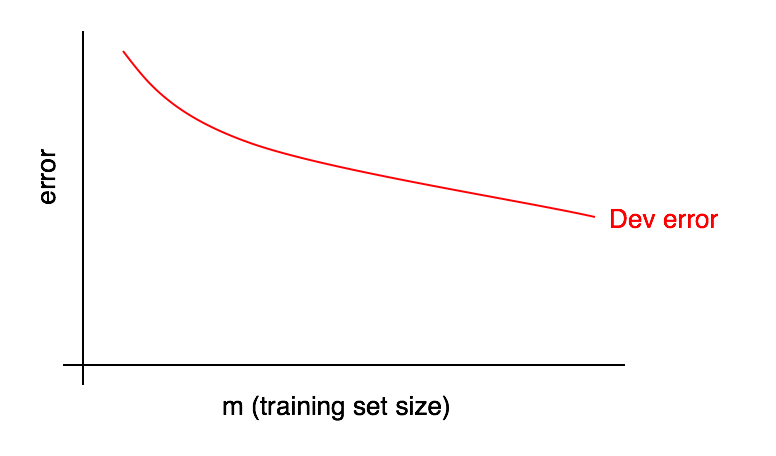
\includegraphics{./img/ch28_01.jpg}

随着训练集大小的增加,开发集误差应该降低。

我们通常会设置一些``期望错误率'',并希望学习算法最终能够达到该值。例如:

\begin{itemize}
\tightlist
\item
  如果希望算法能达到人类水平的表现,那么人类错误率可能就是``期望错误率''。
\item
  如果学习算法为某些产品提供服务(如提供猫咪图片),我们或许将主观感受到需什么样的水平才能给用户提供出色的体验。
\item
  如果你已经从事一项应用很长时间,那么你可能会有一种直觉,预判在下一个季度里你会有多大的进步。
\end{itemize}

将期望的表现水平添加到你的学习曲线中:

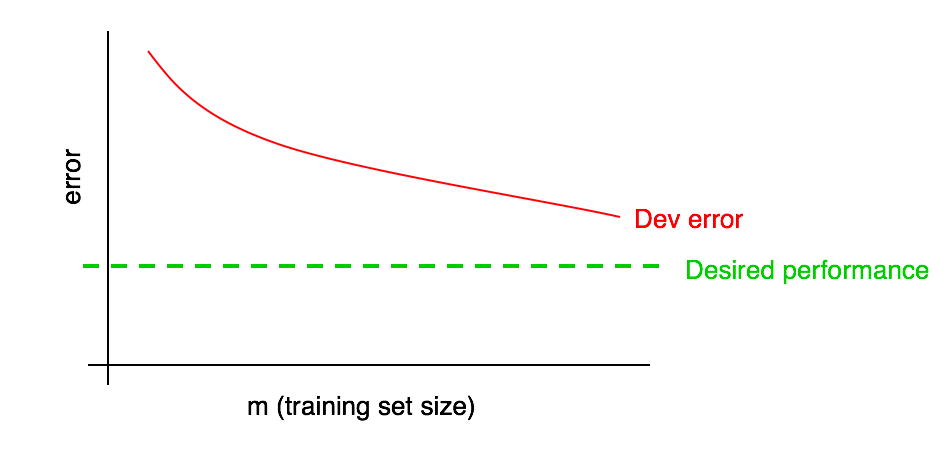
\includegraphics{./img/ch28_02.jpg}

显而易见,你可以根据红色的``开发误差''曲线的走势来推测,在添加一定量的数据后,曲线距离期望的性能接近了多少。在上面的例子中,将训练集的大小增加一倍可能会让你达到期望的性能,这看起来是合理的。

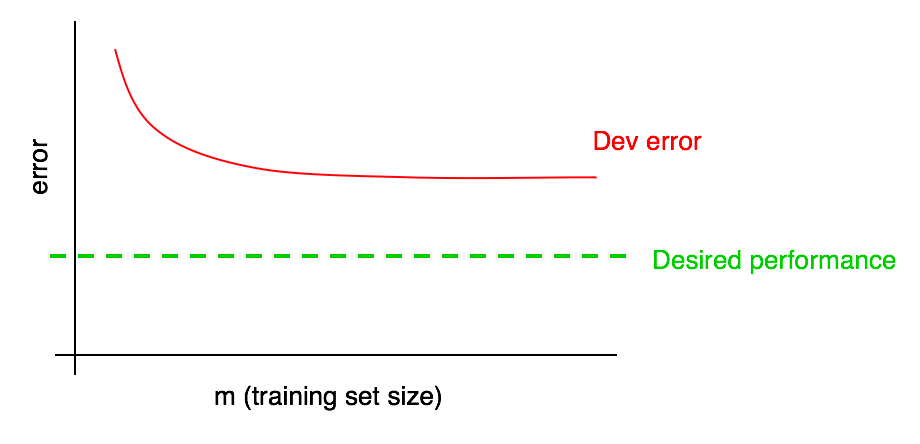
\includegraphics{./img/ch28_03.jpg}

因此,观察学习曲线或许能帮到你,避免了花费几个月的时间去收集两倍的训练数据,到头来却发现这并不管用的情况。

该过程的一个缺点是,如果你只关注了开发错误曲线,当数据量变得越来越多时,将很难预测后续红色曲线的走向。因此我们会选择另外一条曲线来协助评估添加数据所带来的影响:即训练误差曲线。

\hypertarget{ux7ed8ux5236ux8badux7ec3ux8befux5deeux66f2ux7ebf}{%
\chapter{绘制训练误差曲线}\label{ux7ed8ux5236ux8badux7ec3ux8befux5deeux66f2ux7ebf}}

随着训练集大小的增加,开发集(和测试集)误差应该会降低,但你的训练集误差往往会随之增加。

让我们来举例说明一下。假设你的训练集只有两个样本:一张猫图和一张非猫图。学习算法很轻易地就可以``记住''训练集中这两个样本,并且训练集错误率为
0\%. 即使有一张或两张的样本图片被误标注了,算法也能够轻松地记住它们。

现在假设你的训练集包含 100
个样本,其中有一些样本可能被误标记,或者是模棱两可的(图像非常模糊),所以即使是人类也无法分辨图中是否有一只猫。此时,或许学习算法仍然可以``记住''大部分或全部的训练集,但很难获得
100\% 的准确率。通过将训练集样本数量从 2 个增加到 100
个,你会发现训练集的准确率会略有下降。

下面我们将训练误差曲线添加到原有的学习曲线中:

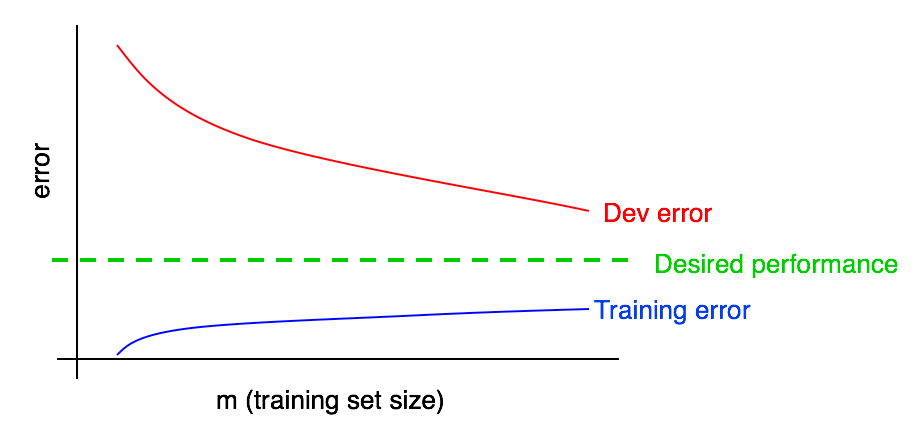
\includegraphics{./img/ch29_01.jpg}

可以看到,蓝色的``训练误差''曲线随着训练集大小的增加而上升,而且算法在训练集上通常比在开发集上表现得更好;因此,红色的开发误差曲线通常严格位于蓝色训练错误曲线之上。

让我们来讨论一下如何解释这些曲线的含义。

\hypertarget{ux89e3ux8bfbux5b66ux4e60ux66f2ux7ebfux9ad8ux504fux5dee}{%
\chapter{解读学习曲线:高偏差}\label{ux89e3ux8bfbux5b66ux4e60ux66f2ux7ebfux9ad8ux504fux5dee}}

假设你的开发误差曲线如下图所示:

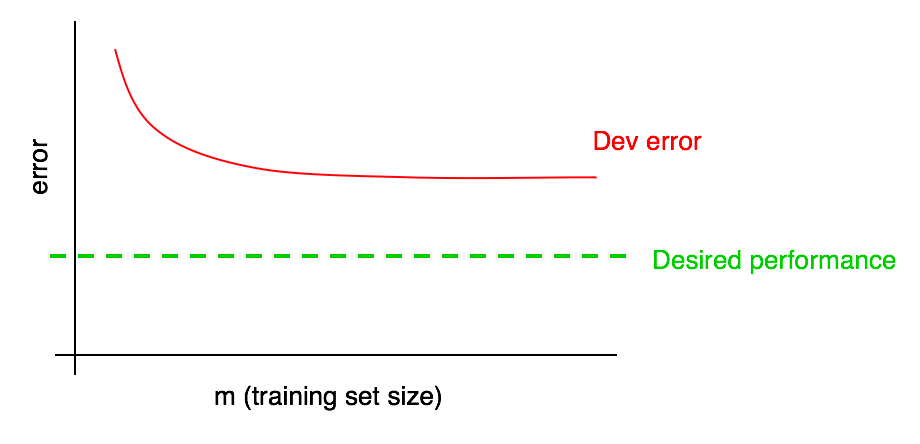
\includegraphics{./img/ch30_01.jpg}

我们之前提到,如果开发误差曲线趋于平稳,则不太可能通过添加数据来达到预期的性能,但也很难确切地知道红色的开发错误曲线将趋于何值。如果开发集很小,或许会更加不确定,因为曲线中可能含有一些噪音干扰。

假设我们把训练误差曲线加到上图中,可以得到如下结果:

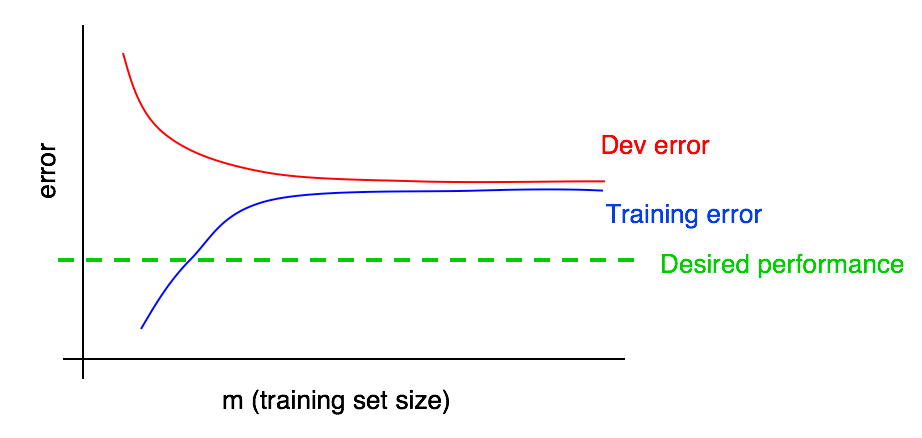
\includegraphics{./img/ch30_02.jpg}

现在可以绝对肯定地说,添加更多的数据并不奏效。为什么呢?记住我们的两个观察结果:

\begin{itemize}
\tightlist
\item
  随着我们添加更多的训练数据,训练误差变得更糟。因此蓝色的训练误差曲线只会保持不动或上升,这表明它正远离期望的性能水平(绿色的线)。
\item
  红色的开发误差曲线通常要高于蓝色的训练误差曲线。因此只要训练误差高于期望性能,通过添加更多数据来让红色开发误差曲线下降到期望性能水平之下也基本没有可能。
\end{itemize}

在同一张图中检查开发误差曲线和训练误差曲线可以让我们对推测开发误差曲线的走势更有信心。

为了便于讨论,假设期望性能是我们对最优错误率的估计。那么上面的图片就是一个标准的``教科书''式的例子(具有高可避免偏差的学习曲线是什么样的):在训练集大小的最大处(大致对应使用我们所有的训练数据),训练误差和期望性能之间有较大的间隙,这代表可避免偏差较大。此外,如果训练曲线和开发曲线之间的间隙小,则表明方差小。

之前,我们只在曲线最右端的点去衡量训练集误差和开发集误差,这与使用所有的可训练数据训练算法相对应。绘制完整的学习曲线将为我们呈现更全面的结果图片,显示算法在不同训练集大小上的表现。

\hypertarget{ux89e3ux8bfbux5b66ux4e60ux66f2ux7ebfux5176ux5b83ux60c5ux51b5}{%
\chapter{解读学习曲线:其它情况}\label{ux89e3ux8bfbux5b66ux4e60ux66f2ux7ebfux5176ux5b83ux60c5ux51b5}}

考虑下面的学习曲线:

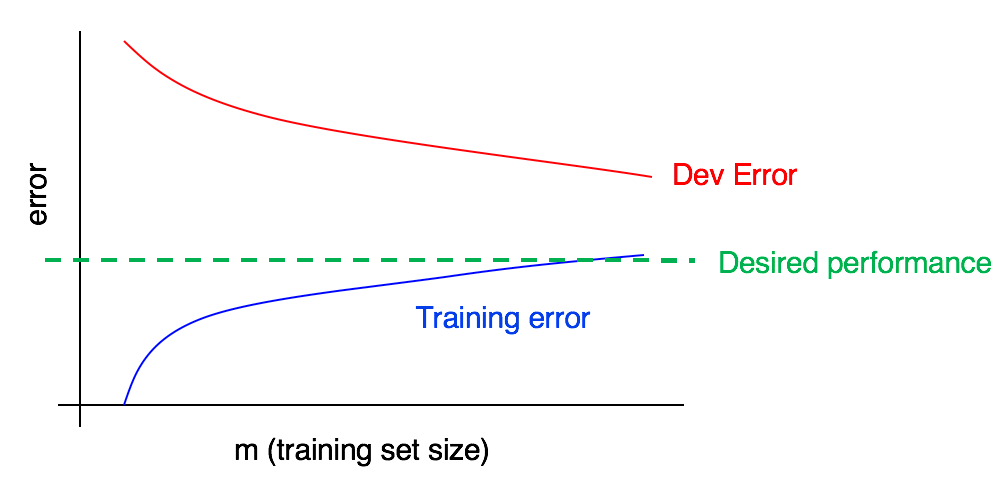
\includegraphics{./img/ch31_01.jpg}

这张图表示的是高偏差?高方差?还是两者都有?

蓝色训练误差曲线相对较低,红色的开发误差曲线比蓝色训练误差高得多。因此,偏差很小,但方差很大。添加更多的训练数据可能有助于缩小开发误差和训练误差之间的差距。

现在考虑下面的情况:

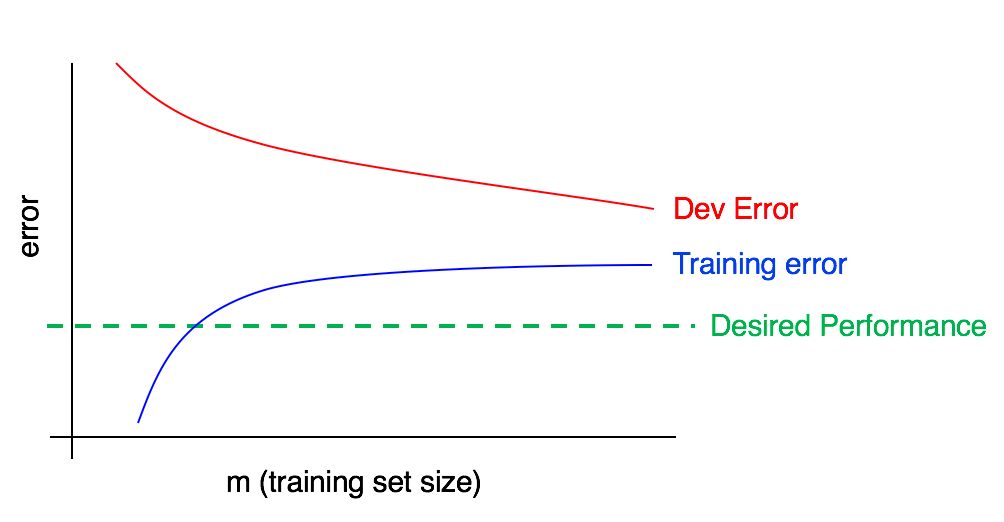
\includegraphics{./img/ch31_02.jpg}

这种情况下,训练误差很大,它比期望的性能水平要高得多,开发误差也比训练误差大得多。因此,学习算法有着明显的偏差和方差。此时你必须找到一种方法来减少算法中的偏差和方差。

\hypertarget{ux7ed8ux5236ux5b66ux4e60ux66f2ux7ebf}{%
\chapter{绘制学习曲线}\label{ux7ed8ux5236ux5b66ux4e60ux66f2ux7ebf}}

假设你有一个非常小的训练集,仅有 100 个样本 。那么你可以从中随机选择 10
个样本来训练你的算法,然后是 20 个,30 个,100 个,每次增加 10
个样本。然后使用 10
个数据点来绘制你的学习曲线。你可能会发现,在较小规模的训练集上,曲线看起来带有点噪声(这意味着这些值比预期的要高/低)。

当只使用 10
个随机选择的样本进行训练时,你可能会不幸碰到特别``糟糕''的训练集,比如含有很模糊的或者误标记的样本。你当然也有可能会幸运地碰到特别``棒''的训练集。训练集的规模较小意味着开发和训练误差将随机波动。

如果你的机器学习应用程序很倾向于某一个类(如猫分类任务的负面样本比例远远大于正面样本),或者说有大量的类(如识别
100
种不同的动物物种),那么选择一个``非代表性''或糟糕的特殊训练集的几率也将更大
。例如,假设你的整个样本中有 80\% 是负样本(y=0),只有 20\%
是正样本(y=1),那么一个含有 10
个样本的训练集就有可能只包含负样本,因而算法很难从中学到有意义的东西。

存在训练集噪声致使难以正确理解曲线的变化时,有两种解决方案:

\begin{itemize}
\tightlist
\item
  与其只使用 10 个样本训练单个模型,不如从你原来的 100
  个样本中进行随机有放回抽样,选择几批(比如 3-10 )不同的 10
  个样本进行组合。在这些数据上训练不同的模型,并计算每个模型的训练和开发错误。最终,计算和绘制平均训练集误差和平均开发集误差。
\item
  如果你的训练集偏向于一个类,或者它有许多类,那么选择一个``平衡''子集,而不是从
  100 个样本中随机抽取 10 个训练样本。例如,你可以确保这些样本中的
  2/10是正样本,8/10
  是负样本。更常见的做法是,确保每个类的样本比例尽可能地接近原始训练集的总体比例。
\end{itemize}

\begin{quote}
此处\textbf{有放回抽样}的意思是:你会从 100 个样本中随机选择 10
个不同的样本来生成第一个训练集,在生成第二个训练集时,你需要再次选择 10
个样本,且抽样来源仍需包括第一次选择的 10
个样本在内。因此,某一个样本可能在第一个训练集和第二个训练集都有出现。相反,如果你在无放回的情况下进行抽样,那么第二个训练集将从第一次没有被选择的
90
个样本中选出。在实践中,用有放回抽样和无放回抽样的差异不大,但是前者更为常见。
\end{quote}

除非你已经尝试过绘制学习曲线,并得出了曲线太过嘈杂且无法看到潜在趋势的结论,否则我将不会考虑使用这两种技术。因为当你的训练集规模很大------比如超过
10000 个样本------而且类分布不是很倾斜时,你可能就不需要这些技巧了。

最后提一点,绘制一个学习曲线的成本可能非常高:例如,你可能需要训练 10
个模型,其中样本规模可以是 1000 个,然后是 2000 个,一直到 10000
个。使用小数据集训练模型比使用大型数据集要快得多。因此,你可以用
1000、2000、4000、6000 和 10000
个样本来训练模型,而不是像上面那样将训练集的大小均匀地间隔在一个线性的范围内。这仍然可以让你对学习曲线的变化趋势有一个清晰的认识。当然,这种技术只有在训练所有额外模型所需的计算成本很重要时才有意义。

\hypertarget{ux4e0eux4ebaux7c7bux8868ux73b0ux6c34ux5e73ux5bf9ux6bd4}{%
\part{与人类表现水平对比}\label{ux4e0eux4ebaux7c7bux8868ux73b0ux6c34ux5e73ux5bf9ux6bd4}}

\hypertarget{ux4e3aux4f55ux4e0eux4ebaux7c7bux8868ux73b0ux6c34ux5e73ux8fdbux884cux5bf9ux6bd4}{%
\chapter{为何与人类表现水平进行对比}\label{ux4e3aux4f55ux4e0eux4ebaux7c7bux8868ux73b0ux6c34ux5e73ux8fdbux884cux5bf9ux6bd4}}

许多机器学习系统的设计目的是想要自动化一些人类可以处理得很好的事情,可举的例子有图像识别、语音识别以及垃圾邮件分类等等。学习算法进步如此之快,有许多类似任务的处理已经超过了人类的表现水平。

此外,有许多理由表明在处理人类擅长的任务时,构建一个机器学习系统会更加简单:

\begin{enumerate}
\def\labelenumi{\arabic{enumi}.}
\tightlist
\item
  \textbf{易于从人为标签中获取数据。}举个例子,由于人类可以很好地识别图片中的猫,因此让人们为你的学习算法提供高精度的带标签数据也很方便。
\item
  \textbf{基于人类直觉进行误差分析。}假设某个语音识别系统的表现要低于人类的表现水平。比如错误地将音频片段
  ``This recipe calls for a \emph{pear} of apples'' 中的 ``\emph{pair}''
  认为是 ``\emph{pear}''.
  此时你可以利用人类的直觉来尝试理解,普通人会利用何种信息来获取正确的转录内容,并且试着修改你的学习算法,使它在相同的知识点上有着更好的表现。
\item
  \textbf{使用人类表现水平来估计最优错误率,并设置可达到的``期望错误率''。}
  假设你的算法在某个任务上达到了 10\% 的误差,但普通人所能达到的误差是
  2\% . 由此我们就可以知道最优错误率是 2\%
  或更低,这也表明可避免偏差至少是 8\% .
  所以你应当尝试一下降低偏差的技术。更一般地说,有一个合理可实现的``期望错误率''可以帮助你去估计学习算法的可避免偏差。这反过来也帮你决定是否使用误差降低技术。
\end{enumerate}

尽管第三点可能听起来不太重要,但我发现有一个合理且可实现的目标错误率有助于加快团队的进度。知道你的算法有很高的可避免偏差是非常有价值的,它将展开一个具有多个选项的菜单供你去尝试。

连人类都不擅长的任务也是存在的。比如向你推荐一本书,或者在某个网站上选择向用户展示的广告,或者对股票市场进行预测。如今计算机在此类任务上的表现已经远超过人类。对于这些应用,我们主要面临着下面的问题:

\begin{itemize}
\tightlist
\item
  \textbf{获取标签数据很难。}
  比如很难去获取用户数据库,并要求人工标记者使用``最优''的书籍标签对数据库进行注释,从而向用户推荐书籍。如果你正在负责一个书籍销售网站或者是
  APP
  的运营,你可以通过向用户展示书籍并查看他们的购买记录来获取数据。可当你没有这样一个网站时,就需要去找到一些更具创意的方法来获取数据了。
\item
  \textbf{人类的直觉难以依靠。}例如,几乎没有人能准确地预测股票市场。因此当我们的股票预测算法比随机猜测的表现还要差时,很难弄清楚要如何去改进它。
\item
  \textbf{最优错误率和合理的期望错误率难以确定。}假设你已经有了一个很好的图书推荐系统。如果没有人类水平作为参考,你怎么知道它还能改善多少呢?
\end{itemize}

\hypertarget{ux5982ux4f55ux5b9aux4e49ux4ebaux7c7bux8868ux73b0ux6c34ux5e73}{%
\chapter{如何定义人类表现水平}\label{ux5982ux4f55ux5b9aux4e49ux4ebaux7c7bux8868ux73b0ux6c34ux5e73}}

假设你正在做一个医学成像应用程序,它可以自动依据X射线图像进行诊断。
除了一些基础的训练外,一个没有任何医学背景的人在该任务上的错误率为 15\%
. 一名新手医生的错误率为 10\% ,而经验丰富的医生可以达到 5\% .
如果由小型的医生团队对每一幅图像进行单独的讨论,错误率将降低至 2\% .
上述的哪一种错误率可以定义为``人类表现水平''呢?

在该情景下,我将使用 2\% 作为人类表现水平的代表来获得最优错误率。
你还可以将 2\%
设置为期望的性能水平,因为与人类表现水平相比,前一章的所有三个理由都适用:

\begin{itemize}
\tightlist
\item
  \textbf{易于从人为标签中获取数据。}你可以让一组医生为你提供错误率为
  2\% 的标签。
\item
  \textbf{基于人类直觉进行误差分析。}通过与医生讨论图像内容,你可以利用他们的直觉。
\item
  \textbf{使用人类表现水平来估计最优错误率,并设置可达到的``期望错误率''。}
  使用 2\%
  的误差作为我们对最优错误率的估计是合理的。最优错误率甚至可能低于
  2\%,但它不可能更高,因为一个医生团队就已经有可能达到 2\%
  的误差水平。相比之下,使用 5\% 或 10\%
  作为最优错误率的估计就显得不合理了,因为我们知道这些估算值必然过高了。
\end{itemize}

当需要获得标签数据时,你可能不希望与整个团队讨论每一张图片,因为他们的时间很宝贵。或许你可以让新手医生给绝大多数的病例贴上标签,而把那些较难分析的病例交给更有经验的医生或医生团队。

如果你的系统目前的误差为 40\%,那么不论是让初级医生(10\%
误差)还是有经验的医生(5\%
误差误)来给你的数据贴上标签,那都没有关系。是如果你的系统误差已经是
10\%,那么将人类表现水平定义为 2\% 将为你提供更好的途径来改进你的系统。

\hypertarget{ux8d85ux8d8aux4ebaux7c7bux8868ux73b0ux6c34ux5e73}{%
\chapter{超越人类表现水平}\label{ux8d85ux8d8aux4ebaux7c7bux8868ux73b0ux6c34ux5e73}}

现在你在做一个语音识别项目,并且有一个音频片段数据集。假设数据集里有许多的噪声,导致即使是人类来识别也会有
10\% 的误差。同时假设你的算法已经达到了 8\% 的误差,你能够使用第 33
章中提到的三种技术来继续取得快速的进展吗?

如果你能找到人类表现水平远超现有系统的数据子集,使用那些技术来驱动进则仍然可行。举个例子,假设你的系统在处理识别含有噪音的音频任务时表现已经优于人类,然而在转录语速很快的语音时人类仍然占有优势。

对于语速很快的语音数据子集:

\begin{enumerate}
\def\labelenumi{\arabic{enumi}.}
\tightlist
\item
  你仍可以从输出质量比你的算法高的人那儿获取转录数据。
\item
  你可以利用人类的直觉来理解,为什么你的系统没能够识别这些数据,而人类做到了。
\item
  你可以使用该子集上的人类表现水平作为期望表现目标。
\end{enumerate}

更常见的做法是,只要在开发集上存在着一些人类能正确处理而算法不能的样本,前面提到的技术就能够被应用。即使你的算法在整个开发集或是测试集上的表现已经超过了人类,这样做也是正确的。

在许多重要的机器学习应用程序中,机器已经超越了人类的水平。例如,机器可以更好地预测电影分级,一辆送货车到某个地方需要多长时间,或者是否批准贷款申请。只有当人类很难识别出算法明显出错的样本时,一小部分技术才可以被应用。因此在机器已经超越人类水平的问题上,进展通常比较慢,而当机器仍在试图赶上人类水平时,进展速度反而更快。

\hypertarget{ux5728ux4e0dux540cux7684ux5206ux5e03ux4e0aux8badux7ec3ux4e0eux6d4bux8bd5}{%
\part{在不同的分布上训练与测试}\label{ux5728ux4e0dux540cux7684ux5206ux5e03ux4e0aux8badux7ec3ux4e0eux6d4bux8bd5}}

\hypertarget{ux4f55ux65f6ux5728ux4e0dux540cux7684ux5206ux5e03ux4e0aux8badux7ec3ux4e0eux6d4bux8bd5}{%
\chapter{何时在不同的分布上训练与测试}\label{ux4f55ux65f6ux5728ux4e0dux540cux7684ux5206ux5e03ux4e0aux8badux7ec3ux4e0eux6d4bux8bd5}}

假设用户已经向你的猫咪图片程序上传了 10000
张图片,且图片已被人为标记为含有猫与不含猫两类。同时你也从互联网上下载了规模更大的
200000 张图片集,此时训练集、测试集与开发集应该如何定义呢?

由于用户的 10000
张图片密切地反映了你想要处理的数据的实际概率分布,因此你可以将它们作为开发集与测试集。如果你正在训练一个数据量饥渴的深度学习算法,则可能需要使用额外的
200000
张网络图片来进行训练。这样的话,你的训练集与开发集/测试集将服从不同的概率分布。这对你的工作会有什么影响呢?

除了将数据集直接划分为训练集、开发集和测试集这一做法外,我们还能将所有的
210000
张已有图片先进行整合,接着随机打乱它们,再进行划分。经过这样的处理,所有的数据都将服从相同的分布。但我建议你不要使用这种方法,因为这样大约
97.6\%(205,000/210,000)的开发/测试数据将来自于互联网图像,这并不能反映出你想要处理数据的实际分布。请记住我们关于选择开发/测试集的建议:

\begin{quote}
选择开发集和测试集以反映你在将来想要正确处理的数据。
\end{quote}

大多数关于机器学习的学术文献都假定训练集、开发集和测试集都来自于相同的分布。在机器学习的早期,数据是稀缺的。我们通常只有一个服从某些概率分布的数据集。因此,我们会随机地将这些数据分割成训练/开发/测试集,并且假设所有的数据来源相同且满足要求。

\begin{quote}
有一些在不同的分布上进行训练和测试的学术研究。例子包括``域适应''、``迁移学习''和``多任务学习''。但理论与实践之间仍存在巨大差距。如果你在数据集A上进行训练,并测试一些类型很不一样的数据B,运气成分可能会对你的算法的性能产生巨大的影响。(在这里,``运气''包括了研究人员为特定任务人为设计的特征,以及其他我们还不了解的因素。)这使得对不同分布的训练和测试的学术研究难以系统地进行。
\end{quote}

但在大数据时代,我们现在可以使用大型的训练集,比如猫的网络图像。即使训练集的分布不同,我们仍然希望使用它来学习,因为它可以提供大量的信息。

对于猫咪检测器的示例,我们不会将用户上传的所有 10000
个图像放到开发/测试集合中,而是将其中 5000 张放入。 这样的话,训练集中的
205000 个样本的分布将来自现有的开发/测试集,以及 200000
张网络图片。我们将在后面的章节中讨论为什么这个方法是有帮助的。

让我们考虑第二个例子。假设你正在建立一个语音识别系统,将某个街道地址转换为一个语音控制的移动地图/导航应用程序。现在你有
20000 个``用户说出街道地址''的样本,但是你也有 500000
个其他音频片段的样本,内容是``用户谈论其他话题''。你可能会为开发/测试集合选取
10000 个街道地址样本,并使用剩下的 10000 个样本,再加上 50
万个其它音频内容的样本进行训练。

我们将继续假设你的开发数据和测试数据来自相同的分布。但重要的是你要明白,不同的训练和开发/测试集分布将带来一些特殊的挑战。

\hypertarget{ux5982ux4f55ux51b3ux5b9aux662fux5426ux4f7fux7528ux4f60ux6240ux6709ux7684ux6570ux636e}{%
\chapter{如何决定是否使用你所有的数据}\label{ux5982ux4f55ux51b3ux5b9aux662fux5426ux4f7fux7528ux4f60ux6240ux6709ux7684ux6570ux636e}}

假设你的猫咪检测器的训练集包括 10000
张用户上传的图片,这些数据来自相同的数据分布且将作为单独的开发/测试集,同时也代表着你关心的将要处理的数据分布。你还从互联网下载了额外的
20000 张图片。此时你是否应该为你的学习算法提供所有的 20000 + 10000
张图片作为它的训练集,或者丢弃这 20000
张网络图片,以免它会影响你的学习算法呢?

在使用早期的学习算法(比如人为设计的计算机视觉特征,然后使用一个简单的线性分类器)时,真正的风险在于:合并这两种类型的数据会导致算法的表现更差。因此,一些工程师会警告你不要加入
20000 张互联网图片。

但是有了现代强大而灵活的学习算法------比如大型的神经网络------这种风险已经大大降低了。如果你能够构建一个有足够多的隐藏单元/层的神经网络,你可以安全地将
20000 张图片添加到你的训练集。此时添加图片则更有可能提升算法的性能。

这种观察依赖于这样一个事实,即有一些 x-y
映射对于这两种类型的数据都很有效。换而言之,有这么些系统可以输入互联网图像或移动应用上的图像,并可靠地预测标签,即使它不知道图像的来源。

添加额外的 20000 张图片会产生以下影响:

\begin{enumerate}
\def\labelenumi{\arabic{enumi}.}
\tightlist
\item
  它给你的神经网络提供了更多关于猫咪外貌的样本。这是很有帮助的,因为互联网图片和用户上传的移动应用图片确实有一些相似之处。你的神经网络可以将从互联网图像中获得的一些知识应用到移动应用图像中。
\item
  它迫使神经网络花费部分容量来学习网络图像的特定属性(比如更高的分辨率,不同画面结构图像的分布等等)。如果这些属性与移动应用图像有很大的不同,那么它将``耗尽''神经网络的一些表征能力,导致从移动应用图像的分布识别数据的能力就会降低,而这正是你真正关心的东西。从理论上讲,这可能会损害算法的性能。
\end{enumerate}

换一种不同的术语来描述第二个影响,我们可以求助于小说中的人物夏洛克福尔摩斯,他解释道大脑就像一个阁楼;它只有有限的空间。他说,``每增加一个知识,你就会忘记你以前知道的东西。''因此,最重要的是,不要让无用的事实把有用的真相排挤出去。''
(来自阿瑟柯南道尔的《血字的研究》 )

幸运的是,如果你有足够的计算能力来构建一个足够大的神经网络------也就是一个足够大的阁楼------那么这就不是一个严重的问题了。你有足够的能力从互联网和移动应用图像中学习,而不会存在两种类型的数据在容量上的竞争。也即是说,你的算法的``大脑''足够大,不必担心会耗尽阁楼的空间。

但是,如果你没有足够大的神经网络(或者另一个高度灵活的学习算法),那么你应该更加关注训练数据,需要与开发集/测试集的分布相匹配。

如果你认为有些数据没有任何帮助,那么应该将这些数据排除在计算原因之外。例如,假设你的开发/测试集主要包含一些内容是人员、地点、地标、动物的任意图片。同时假设里面有大量的历史文档扫描图片,这些文件不包含任何类似猫的东西。它们看起来和开发/测试集的分布完全不同。没有必要将这些数据作为负样本,因为上述第一个影响带来的好处在这种情况下几乎忽略不计------你的神经网络几乎没有任何东西可以从这些数据中学习,但它们可以应用到开发/测试集中,加入它们将会浪费计算资源和神经网络的表征能力。

\hypertarget{ux5982ux4f55ux51b3ux5b9aux662fux5426ux6dfbux52a0ux4e0dux4e00ux81f4ux7684ux6570ux636e}{%
\chapter{如何决定是否添加不一致的数据}\label{ux5982ux4f55ux51b3ux5b9aux662fux5426ux6dfbux52a0ux4e0dux4e00ux81f4ux7684ux6570ux636e}}

假设你想要学习预测纽约市的房价。考虑房子的大小(输入特征
x),你需要预测价格(目的标签
y)。纽约市的房价非常高。假设你在密歇根州的底特律有第二个住房价格数据集,就会发现那里的房价要低得多。应该把这些数据包含在你的训练集里吗?

房子的大小 x 相同,而价格 y
明显不同,这取决于它是在纽约还是在底特律。如果你只关心预测纽约市的房价,把这两个数据集放在一起会影响算法的表现。在这种情况下,最好忽略不一致的底特律数据。

\begin{quote}
有一种方法可以解决底特律的数据与纽约市数据不一致的问题,即在每一个显示城市的训练样本中增加一个额外的特征。给定一个输入
x ------代表所在的城市------ 此时目标值 y
是明确的。然而在实践中,我并不经常看到这种情况。
\end{quote}

纽约和底特律的样本与移动应用和互联网猫图片的样本有什么不同?

猫咪图像的样本和这有点不一样,因为给定一个输入图片 x
,你能可靠地预测出标签 y
(是否有猫),即使不知道图像是网络图像还是移动应用图像。即有一个函数
f(x)可以从输入 x 映射到目标输出 y ,即使不知道 x 的来源。
因此,从互联网图像中识别的任务与移动应用图像识别的任务是``一致的''。这意味着,将所有的数据包括在内,几乎没有什么负面影响(除了计算成本),甚至还可能有一些积极的作用。相比之下,纽约和底特律的数据则不一致。考虑相同的
x(房子的大小),价格会根据房子的位置而不同。

\hypertarget{ux7ed9ux6570ux636eux52a0ux6743ux91cd}{%
\chapter{给数据加权重}\label{ux7ed9ux6570ux636eux52a0ux6743ux91cd}}

假设你有 20 万张来自互联网的图片,还有来自移动应用用户的 5000
张照片。数据集的大小之间有一个 40:1
的比率。从理论上讲,只要你建立了一个庞大的神经网络,并在所有 205000
张图片上进行足够长的时间训练,那么在网络图像和移动图像上将算法都训练得很好是没有害处的。

但在实际操作中,拥有 40 倍的网络图像可能意味着,相比只使用 5000
张图片,你需要花费 40 倍(或更多)的计算资源来对两者进行建模。

如果你没有巨大的计算资源,你可以给互联网图片一个较低的权重作为妥协。

例如,假设优化目标是平方误差(对于分类任务来说这不是一个好的选择,但它将简化解释过程)。因此,我们的学习算法试图优化:

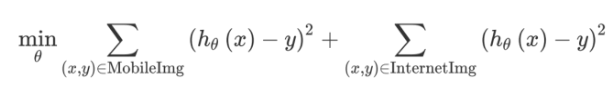
\includegraphics{./img/ch39_01.png}

上面的第一个项是对 5000 个移动应用图像误差求和,第二项对 20
万个互联网图像误差求和。你可以使用一个额外的参数 𝛽 进行优化:

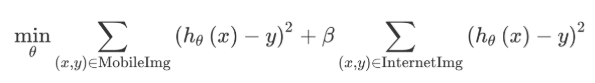
\includegraphics{./img/ch39_02.png}

如果你设置 𝛽 = 1/40,这个算法会对 5000 个移动图像和 20
万个互联网图像给予同等的权重。你还可以将参数 𝛽
设置为其他值,也可以类似地对开发集进行调优。

通过对额外的网络图像赋予更少的权重,你不需要构建一个庞大的神经网络来确保算法在这两种类型的任务上都能很好地完成。只有当你怀疑这些额外的数据(网络图像)与开发/测试集分布不一致,或者额外的数据规模比与相同分布的开发/测试集(手机图像)数据规模大得多时,这种类型的权重加权才需要。

\hypertarget{ux4eceux8badux7ec3ux96c6ux6cdbux5316ux5230ux5f00ux53d1ux96c6}{%
\chapter{从训练集泛化到开发集}\label{ux4eceux8badux7ec3ux96c6ux6cdbux5316ux5230ux5f00ux53d1ux96c6}}

假设你正在将机器学习应用于不同分布的训练集和开发/测试集上。例如,训练集包含了互联网图像+移动应用图像,而开发/测试集只包含移动应用图像。然而,该算法运行得不太好:它的开发/测试集误差比想要的要高得多。以下是一些可能出现问题的情况:

\begin{enumerate}
\def\labelenumi{\arabic{enumi}.}
\tightlist
\item
  它在训练集上表现不佳,这属于训练集分布上的高(可避免)偏差的问题。
\item
  它在训练集上做得很好,但是不能很好地泛化到与训练集分布相同的未知数据,这是高方差问题。
\item
  它能够很好地泛化到与训练集相同分布的未知数据,但不能很好地泛化到与开发/测试集相同分布的未知数据。我们将这种情况称之为\textbf{数据不匹配},因为训练集的数据与开发/测试集的数据匹配得相当地糟糕。
\end{enumerate}

例如,假设人类在猫识别任务上取得近乎完美的表现。你的算法实现了:

\begin{itemize}
\tightlist
\item
  1\% 的训练集误差
\item
  1.5\% 的与训练集分布相同的未知数据上的误差
\item
  10\% 的开发集误差
\end{itemize}

在这种情况下,显然存在着数据不匹配问题。为了解决这个问题,你可能会尝试使训练数据更类似于开发/测试数据。我们稍后将讨论一些相关技术。

为了诊断一个算法在上面 1 到 3
个问题受到了多大程度的影响,存在另一个数据集将是很有用的。具体地说,与其给算法提供所有可用的训练数据,你还可以把它分成两个子集:算法将进行训练的实际训练集,以及一个单独的集合,我们称之为``训练开发''集,我们将不会对它进行训练。

你现在有四个数据子集:

\begin{itemize}
\tightlist
\item
  训练集:这是算法将学习的数据(例如,互联网图像+移动应用图像)。这并不需要我们从与真正关心的相同分布(开发/测试集分布)的数据中提取。
\item
  训练开发集:这些数据来自与训练集相同的分布(例如,互联网图像+移动应用图像)。它通常比训练集要小;它只需要足够大到来评估和跟踪我们的学习算法的进展。
\item
  开发集:这是从与测试集相同分布的数据中抽取出来的,它反映了我们最终关心的数据的分布(例如,移动应用图像)
  。
\item
  测试集:这是从与开发集相同分布的数据中抽取出来的(例如,移动应用图像)。
\end{itemize}

有了这四个独立的数据集,你现在可以评估:

\begin{itemize}
\tightlist
\item
  训练误差,对训练集进行评估。
\item
  该算法能够泛化到与训练集相同分布数据的能力,并对训练开发集进行评估。
\item
  算法在你实际关心的任务上的性能,通过对开发集 和/或 测试集评估。
\end{itemize}

在第 5-7 章中,用于选择开发集大小的大多数指导原则也适用于训练开发集。

\hypertarget{ux8fa8ux522bux504fux5deeux65b9ux5deeux548cux6570ux636eux4e0dux5339ux914dux8befux5dee}{%
\chapter{辨别偏差、方差和数据不匹配误差}\label{ux8fa8ux522bux504fux5deeux65b9ux5deeux548cux6570ux636eux4e0dux5339ux914dux8befux5dee}}

假设在猫咪检测任务中,人类获得了近乎完美的性能(0\%误差),因此最优错误率大约为
0\%。假设你有:

\begin{itemize}
\tightlist
\item
  1\% 的训练集误差
\item
  5\% 的训练开发集误差
\item
  5\% 的开发集误差
\end{itemize}

这表明了什么?你知道你有很高的方差。先前章节描述的减少方差的技术应该能使你取得进展。

现在,假设你的算法达到了:

\begin{itemize}
\tightlist
\item
  10\% 的训练集误差
\item
  11\% 的训练开发集误差
\item
  12\% 的开发集误差
\end{itemize}

这表明你在训练集上有很高的可避免偏差。该算法在训练集上做得很差,偏差降低技术应该能有所帮助。

在上面的两个例子中,该算法只存在高可避免偏差或高方差。一个算法有可能同时受到高可避免偏差、高方差和数据不匹配的子集的影响。例如:

\begin{itemize}
\tightlist
\item
  10\% 的训练集误差
\item
  11\% 的训练开发集误差
\item
  20\% 的开发集误差
\end{itemize}

该算法存在高可避免偏差和数据不匹配问题。然而,它在训练集的分布上并没有很大的差异。
通过将不同类型的误差理解为表中的条目,可能将更容易理解不同类型的误差是如何相互关联的:

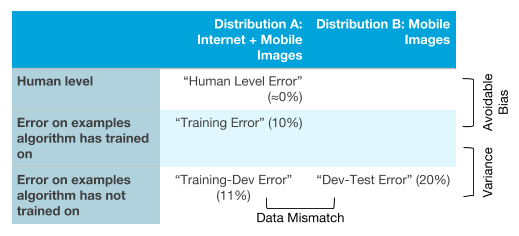
\includegraphics{./img/ch41_01.png}

继续以猫咪图像检测器为例,你可以看到在 x 轴上有两种不同的数据分布。在 y
轴上,我们有三种类型的误差:人为误差,算法上误差,以及算法未经过训练的样本误差。我们可以用我们在前一章中发现的不同类型的误差来填写表格。

如果你愿意,你也可以在这个表格中填入剩下的两个空格:你可以通过让一些人给你的手机图片数据贴上标签,并测量他们的误差,你可以填写右上角的空格(移动应用图像上的人类水平表现)。你也可以通过移动应用猫的图像(分布B)来填充下一个空格,并将一小部分放入训练集,这样神经网络也可以学习它。
然后在数据的子集上测量学习模型的误差。填充这两个额外的条目可能会让我们对算法在两个不同的分布(分布A和B)上做的事情有更多的了解。

通过了解算法最容易产生哪些类型的误差,你将能够更好地决定是否聚焦于减少偏差、减少方差或减少数据不匹配的技术。

\hypertarget{ux89e3ux51b3ux6570ux636eux4e0dux5339ux914dux95eeux9898}{%
\chapter{解决数据不匹配问题}\label{ux89e3ux51b3ux6570ux636eux4e0dux5339ux914dux95eeux9898}}

假设你已经开发了一个语音识别系统,它在训练集和训练开发集上都做得很好。但是,它在你的开发集上做得很差:这表明有一个数据不匹配的问题。你会怎么做呢?

我建议你:(I)尝试理解数据属性在训练集和开发集分布之间的差异。(ii)尝试找到更多的训练数据,以便更好地匹配你的算法碰到的开发集样本。

\begin{quote}
也有一些关于``域适应''的研究------如何在一个分布上训练算法,并将其推广到不同的分布。这些方法通常只适用于特殊类型的问题,并且用得比本章中所描述的理论要少得多。
\end{quote}

例如,假设你在语音识别的开发集中进行误差分析:手动地遍历 100
个样本,并尝试理解算法错出在哪。你会发现你的系统做得的确很差,因为在开发集中,大部分的音频剪辑都是在一辆车里录制的,而大多数的训练样本都是在一个安静的环境下录制的。引擎和道路噪音极大地恶化了你的语音系统的性能。在这种情况下,你可能会尝试获得更多的训练数据,包括在汽车里拍摄的音频片段。误差分析的目的是了解训练集和开发集之间的显著差异,这正是导致数据不匹配的原因。

不幸的是,这个过程没有任何保证。例如,如果你没有任何方法获得更多的训练数据,来更好地匹配开发集数据,那么你可能没有一条明确的路径来提高性能。

\hypertarget{ux4ebaux5de5ux5408ux6210ux6570ux636e}{%
\chapter{人工合成数据}\label{ux4ebaux5de5ux5408ux6210ux6570ux636e}}

你的语音系统需要更多的数据,它们听起来就像是从车里录制得到的。与其在开车的时候收集大量的数据,不如通过人工合成数据来获取这些数据。

假设你获得了大量的汽车/道路噪音的音频剪辑。你可以从几个网站下载这些数据。假设你也有一群在安静的房间里说话的人。如果你把一个人的音频片段``添加''到一个汽车/道路噪音的音频片段,你会得到一个音频剪辑,听起来就好像那个人在嘈杂的汽车里说话一样。使用这个过程,你可以``合成''大量的数据,听起来就像是在汽车里收集的。

更一般的情况是,在一些情况下,人工合成数据允许你创建一个与开发集相当匹配的巨大数据集,让我们使用猫咪图像检测器作为第二个例子。你注意到,开发集的图像有更多的动态模糊,因为它们往往来自手机用户,他们在拍照时会微微地移动手机。你可以从网络图像的训练集中获取非模糊的图像,并将模拟的动态模糊添加到它们中,从而使它们更类似于开发集。

请记住,人工数据合成存在一定的挑战:有时候创建一个对人而言真实的合成数据比创建对计算机而言真实的数据要容易得多。例如,假设你有
1000 小时的语音训练数据,但只有 1 小时的汽车噪音。如果你反复使用相同的 1
小时的汽车噪音,从最初的 1000
小时的训练数据中,你将会得到一个合成的数据集,然而同样的汽车噪音会不断重复。听这段音频的人可能无法分辨------所有的汽车噪音对我们大多数人来说都是一样的------但是某种学习算法可能会``过拟合''一小时的汽车噪音。因此,它可能无法很好地泛化到一个新的音频剪辑片段,里面汽车的噪音听起来是不同的。

另一种情况,假设你有 1000 个小时的汽车噪音片段,但所有的噪音都是从 10
辆不同的车上提取的。在这种情况下,一种算法可能会``过拟合''这 10
辆车,如果在不同的汽车上进行音频测试,性能则会很差。不幸的是,这些问题很难被发现。

再举一个例子,假设你正在建立一个计算机视觉系统来识别汽车:你正与一家电脑游戏公司合作,该公司拥有几辆汽车的计算机图形模型。为了训练你的算法,你可以使用这些模型来生成汽车的合成图像。即使合成的图像看起来非常真实,但这种方法(已经被许多人独立提出)可能不会很好地工作。在整个电脑游戏中,可能有
20 种汽车设计。制造一辆汽车的 3D
模型价格是非常昂贵的;如果你在玩这个游戏,你可能不会注意到你正在一遍又一遍地看到同样的车,也许只是换了一种颜色。即这些数据对你来说很真实。但是,与所有在道路上行驶的汽车相比------也就是你可能在开发/测试集里看到的------这组根据
20
辆汽车模型合成的汽车只捕获了世界上销售的汽车的极小一部分。因此,如果你的
10 万个训练样本都来自这 20 辆车,你的系统将会``过拟合''这 20
款特定的汽车设计,而且它将无法很好地泛化到包含其他汽车设计在内的开发/测试集。

当你在合成数据时,请考虑一下你是否真的在合成一组具有代表性的样本。尽量避免给出合成数据的属性,这将使学习算法有可能将合成和非合成的样本区分开来------例如,所有的合成数据是否来自
20
个汽车设计中的某一个,或者所有的合成音频是否都来自于某个小时的汽车噪音。这个建议很容易被忽视。

在处理数据合成过程时,我的团队有时会花上几周的时间来生成带有细节的数据,这些数据与实际的数据分布非常接近,从而产生显著的效果。但如果你能够正确地获取这些细节,你可以突然获得比以前更大的训练集。

\hypertarget{ux8c03ux8bd5ux63a8ux7406ux7b97ux6cd5}{%
\part{调试推理算法}\label{ux8c03ux8bd5ux63a8ux7406ux7b97ux6cd5}}

\hypertarget{ux4f18ux5316ux9a8cux8bc1ux6d4bux8bd5}{%
\chapter{优化验证测试}\label{ux4f18ux5316ux9a8cux8bc1ux6d4bux8bd5}}

假设你正在构建一个语音识别系统,该系统通过输入一个音频片段 \(A​\)
,并为每一个可能的输出句子 \(S​\) 计算得分
\(\text{Score}_A(S)​\)。例如,你可以试着估计\(\text{Score}_A(S)=P(S\|A)​\),表示句子
\(S​\) 是正确输出的转录的概率,其中 \(A​\) 是给定的输入音频。

给定某种方法能够计算\(\text {Score}_A(S)\)后,你仍然需要找到一个英文句子
\(S\) 来使之最大化:

\[
\text{Output} = \arg \max_s \text{Score}_A(S)
\]

要如何去计算上面的 \(\arg \max\) 呢?假设在英文中共有 5000
个词汇,对于长度为 \(N\) 的句子,则有 \(50000^N\)
种搭配,多到根本无法一一列举。因此,你需要使用一种近似搜索算法,努力去找到能够优化(最大化)\(\text{Score}_A(S)\)
的那个 \(S\) . 有一种叫做 ``定向搜索''
的搜索算法,在搜索过程中仅保留最优的 \(K\)
个候选项(在本章中你并不需要了解该算法的细节)。类似这样的算法并不足以保证能够找到满足条件的
\(S\) 来最大化\(\text{Score}_A(S)\) .

假设有一个音频片段记录着某人说的:``我爱机器学习。''但你的系统输出的却是不正确的
``我爱机器人。'',它没能够输出正确的转录。造成该误差的可能原因有两种:

\begin{enumerate}
\def\labelenumi{\arabic{enumi}.}
\tightlist
\item
  \textbf{搜索算法存在问题。}
  近似搜索算法没能够找到最大化\(\text{Score}_A(S)\) 的那个 \(S\) .
\item
  \textbf{目标(得分函数)存在问题。} 我们对
  \(\text{Score}_A (S)=P(S\|A)\)
  的估计并不准确。尤其在此例中,我们的得分函数没能辨认出
  ``我爱机器学习'' 是正确的转录。
\end{enumerate}

对应不同的失败原因,你需要优先考虑的工作方向也将很不一样。如果原因 1
导致了问题,你应该改进搜索算法。如果原因 2
导致了问题,你应该在评估学习算法的函数 \(\text{Score}_A(S)\)
上面多花些心思。

面对这种情况,一些研究人员将决定研究搜索算法;其他人则努力去找到更好的
\(\text{Score}_A(S)\) .
但是,除非你知道其中哪一个是造成误差的潜在原因,否则你的努力可能会被浪费掉。怎么样才能更系统地决定要做什么呢?

让我们用 \(S_{out}\) 表示实际的输出 ``我爱机器人'',用 \(S^*\)
表示正确的输出 ``我爱机器学习'' 。为了搞清楚上面的 1 或 2
是否存在问题,你可以执行 \textbf{优化验证测试(Optimization Verification
test)}: 首先计算 \(S_{out}\) 和 \(S^*\)
,接着比较他们的大小。有两种可能:

情况1:\(\text{Score}\_A {(S^*)} \gt \text{Score}\_A {(S_{out})}\)

在这种情况下,你的学习算法正确地给了 \(S^*\) 一个比 \(S_{out}\)
更高的分数。尽管如此,我们的近似搜索算法选择了 \(S_{out}\) 而不是
\(S^*\) . 则表示你的近似搜索算法没能够找到最大化\(\text{Score}_A(S)\)
的那个 \(S\) .
此时优化验证测试告诉你,搜索算法存在着问题,应该花时间研究。例如,你可以尝试增加定向搜索的搜索宽度。

情况2:\(\text{Score}\_A (S^*) \leq \text{Score}\_A (S_{out})\)

在这种情况下,计算 \(\text{Score}\_A (.)\)
的方式是错误的:它没有给正确的输出 \(S^*\) 比实际输出 \(S_{out}\)
一个相同或更高的分数。优化验证测试告诉你,目标(得分函数)存在问题。因此,你应该专注于改进你的算法对不同的句子
\(S\) 学习或近似出得分 \(\text{Score}_A (S)\) 的方式。

我们上面的讨论集中于某个单一的样本 \(A\)
上,想要在实践中运用优化验证测试,你需要在开发集中检测这些误差样本。对于每一个误差样本,你都需要测试是否有
\(\text{Score}\_A (S^*) \gt \text{Score}\_A (S)\_{out}\) .
开发集中所有满足该不等式的样本都将被标记为优化算法自身所造成的误差,而满足不等式
\(\text{Score}\_A (S^*) \leq \text{Score}\_A (S)_{out}\)
的样本将被记为是计算得分 \(\text{Score}_A (.)\) 造成的误差。

假设你最终发现 95\% 的误差是得分函数 \(\text{Score}_A (.)\)
造成的,而仅有 5\%
的误差是由优化算法造成的。现在你应该知道了,无论你如何改进你的优化程序,
实际上也只会消除误差中的 5\% 左右。因此,你应该专注于改进你的得分函数
\(\text{Score}_A (.)\) .

\hypertarget{ux4f18ux5316ux9a8cux8bc1ux6d4bux8bd5ux7684ux4e00ux822cux5f62ux5f0f}{%
\chapter{优化验证测试的一般形式}\label{ux4f18ux5316ux9a8cux8bc1ux6d4bux8bd5ux7684ux4e00ux822cux5f62ux5f0f}}

你可以在如下情况运用优化验证测试,给定输入 \(x\) ,且知道如何计算
\(\text{Score}_x (y)\) 来表示 \(y\) 对输入 \(x\)
的响应好坏。此外,你正在使用一种近似算法来尽可能地找到\(\arg \max_y \text{Score}_x(y)\)
,但却怀疑该搜索算法有时候并不能找到最大值。在我们先前提到的语音识别的例子中,\(x=A\)
代表某个音频片段, \(y=S\) 代表输出的转录。

假设 \(y^*​\) 是 ``正确的'' 输出,可算法输出了 \(y_{out}​\) .
此时的关键在于测量是否有
\(\text{Score}\_x(y^*) \ge \text{Score}\_x(y\_{out})​\) .
如果该不等式成立,我们便可以将误差归咎于优化算法。(请参考前一章的内容,以确保你理解这背后的逻辑。)否则,我们将误差归咎于
\(\text{Score}_x (y)​\) 的计算方式。

让我们再看一个例子:假设你正在构建一个中译英的机器翻译系统,输入一个中文句子\(C\)
,并计算出每一个可能的翻译句子 \(E\) 的得分
\(\text{Score}_C(E)\),例如,你可以使用
\(\text{Score}_C(E)=P(E\|C)\),表示给定输入句子 \(C\) ,对应翻译句子为
\(E\) 的概率。

你的算法将通过计算下面的公式来进行句子的翻译: \[
\text{Output}=\arg \max_E \text{Score}_C(E)
\]
然而所有可能的英语句子构成的集合太大了,所以你将依赖于启发式搜索算法。

假设你的算法输出了一个错误的翻译 \(E_{out}​\),而不是正确的翻译 \(E^*​\) .
优化验证测试会要求你计算是否有
\(\text{Score}\_C (E^*) \gt \text{Score}\_C (E)_{out}​\) .
如果这个不等式成立,表明 \(\text{Score}_C(.)​\) 正确地辨认 \(E^*​\)
是一个更好的输出;因此你可以将把这个误差归咎于近似搜索算法。否则,你可以将这个误差归咎于
\(\text{Score}_C(.)​\) 的计算方式。

在人工智能领域,这是一种非常常见的
``设计模式'',首先要学习一个近似的得分函数 \(\text{Score}_X(.)\)
,然后使用近似最大化算法。如果你能够发现这种模式,就能够使用优化验证测试来理解造成误差的来源。

\hypertarget{ux5f3aux5316ux5b66ux4e60ux4e3eux4f8b}{%
\chapter{强化学习举例}\label{ux5f3aux5316ux5b66ux4e60ux4e3eux4f8b}}

假设你正在用机器学习来教直升机复杂的飞行动作。下面是一张延时照片,照片上是一台电脑控制器的直升机正在引擎关闭的情况下执行着陆。

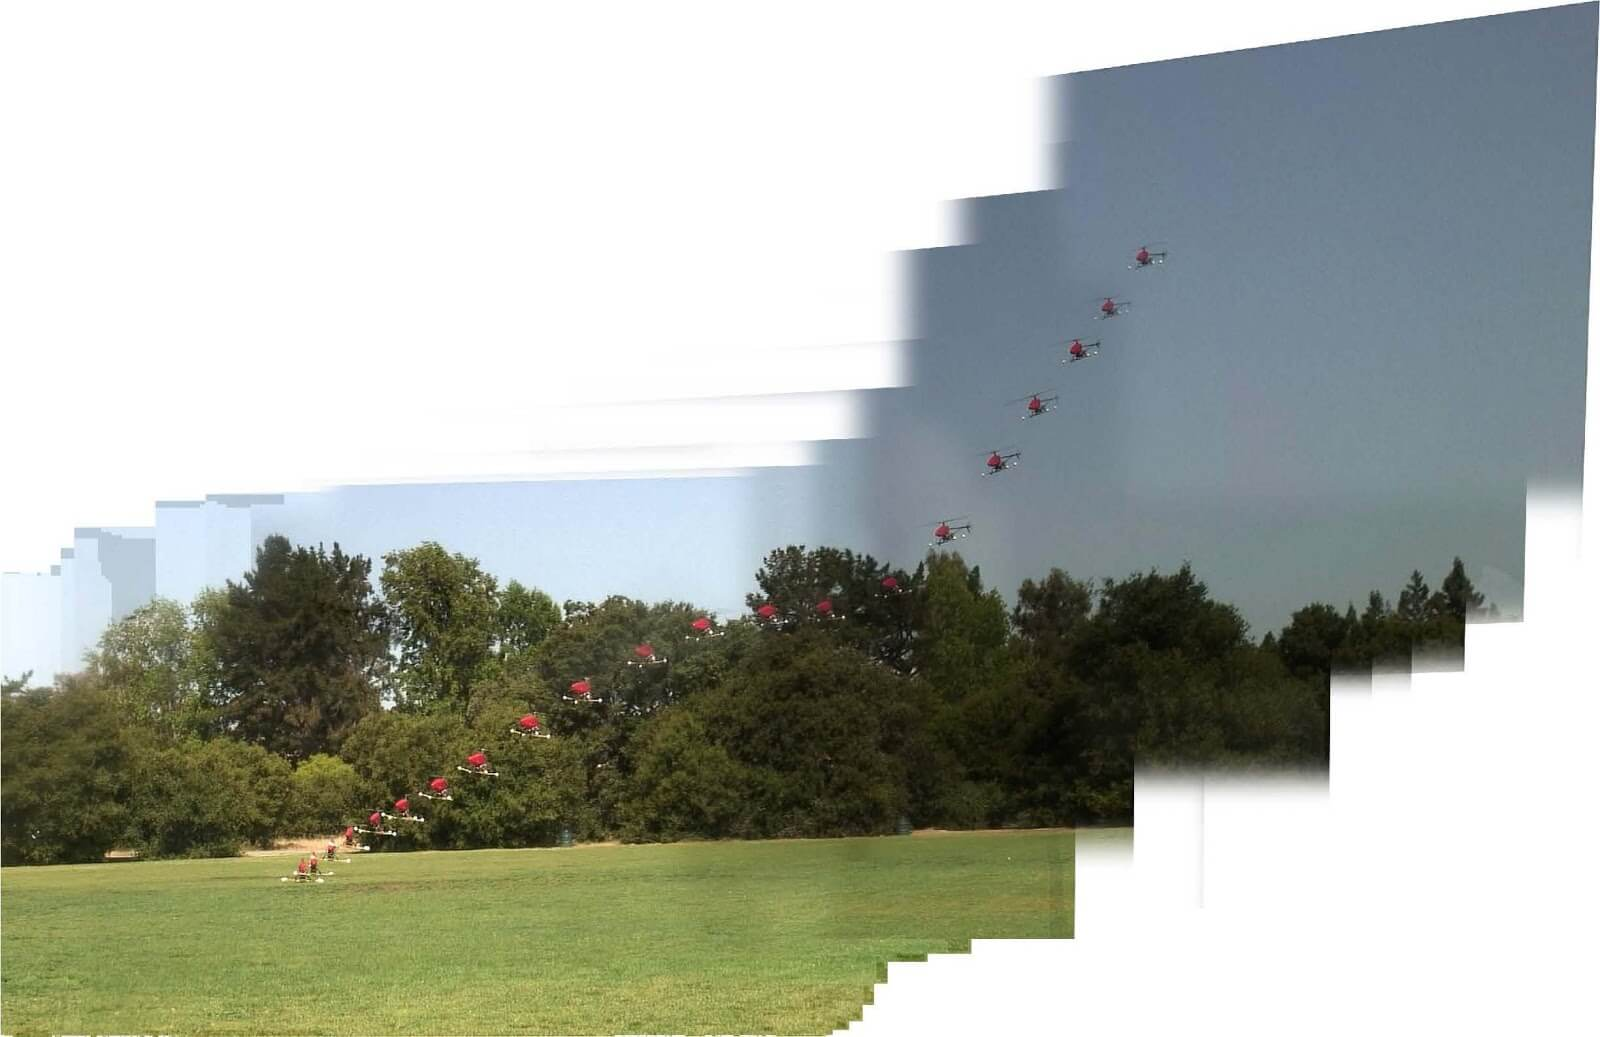
\includegraphics{./img/ch46.jpg}

这被称为``自旋''策略,即使引擎意外故障了,它也允许直升机着陆。这也是人类飞行员经常进行的训练。而你的目标是使用一种学习算法,让直升机通过一个轨迹
\(T\) 安全地着陆。

要应用强化学习策略,你必须设计一个 ``奖励函数''
\(R(.)\),它给出一个分数来衡量每一个可能轨迹 \(T\) 的好坏。例如,如果
\(T\) 导致直升机坠毁,那么奖励也许是 \(R(T)=-1000\)
,这是一个巨大的负反馈;而一个导致安全着陆的轨迹 \(T\)
可能会产生一个正的 \(R(T)\)
值,它的精确值取决于着陆过程的平稳程度。奖励函数 \(R(.)\)
通常是人为选择的,以量化不同轨迹 \(T\)
的理想程度。它必须权衡考虑着陆的颠簸程度,直升机是否降落在理想的位置,乘客的降落体验等因素。设计一个好的奖励函数并非易事。

给定一个奖励函数 \(R(T)\) ,强化学习算法的工作是控制直升机,使其达到
\(\max_TR(T)\) .
然而,强化学习算法原理内部有许多近似操作,可能无法成功实现这种最大化需求。

假设你已经选择了某些奖励函数 \(R(T)\)
作为反馈,并运行了学习算法。然而它的表现似乎比人类飞行员要糟糕得多------它更加颠簸,而且似乎不那么安全。你如何判断错误是否由强化学习算法造成------它试图找到一个轨迹
\(T\) ,满足 \(\max_TR(T)\)
------或者错误来自于你的奖励函数------它尝试衡量并且指定一种在颠簸程度和着陆精度之间权衡的理想结果。

为了应用优化验证测试,让 \(T_{human}\) 表示人类飞行员所选择的轨迹,并让
\(T_{out}\) 代表算法所选择的轨迹。根据我们上面的描述, \(T_{human}\)
是优于 \(T_{out}\) 的发展轨迹。因此,关键的测试点在于:不等式
\(R(T_{human}) \gt R(T_{out})\) 是否成立?

情况1:如果不等式成立,奖励函数 \(R(.)\) 正确地使 \(T_{human}\) 优于
\(T_{out}\) ,但这表明我们的强化学习算法找到的 \(T_{out}\)
仍不够好,花时间去改进算法是很值得的。

情况2:如果上面不等式不成立,而是 \(R(T_{human}) \leq R(T_{out})\) .
这表明 \(R(.)\) 的设计使得理应是更优策略的 \(T_{human}\)
得到了一个更糟的评分。你应当致力于改进 \(R(.)\)
,以更好地获得与良好着陆情况相对应的权衡。

许多机器学习应用程序使用这种优化某个近似的 ``模式'' 来确定得分函数
\(\text{Score}_X(.)\) . 有时没有特定的输入 \(x\) ,形式简化为
\(\text{Score}X(.)\)
。在上面的例子中,得分函数即是奖励函数,\(\text{Score(T)=R(T)}\),而采用的优化算法是强化学习算法,目的是找到好的轨迹\(T\)
.

这和前面的例子有一个区别,那就是,与其比较 ``最优''
输出,不如将其与人类水平的表现进行比较。我们认为,即使 \(T_{human}\)
不是最优的,它也是相当不错的。一般而言,只要有一个比当前学习算法性能更好的输出
\(y^*\) (在这个例子中即是指 \(T_{human}\) ),即使它不是 ``最优''
的,优化验证测试也能够反映改进学习算法与改进得分函数之间哪一个更具前途。

\hypertarget{ux7aefux5230ux7aefux6df1ux5ea6ux5b66ux4e60}{%
\part{端到端深度学习}\label{ux7aefux5230ux7aefux6df1ux5ea6ux5b66ux4e60}}

\hypertarget{ux7aefux5230ux7aefux5b66ux4e60ux7684ux5174ux8d77}{%
\chapter{端到端学习的兴起}\label{ux7aefux5230ux7aefux5b66ux4e60ux7684ux5174ux8d77}}

假设你想要构建一个系统来对产品的线上评论进行检查,并且要能够自动地告诉你给出评论的人是否喜欢这个产品。比如说,你希望系统将下面的句子识别为十分正面的评论:

\begin{quote}
这个拖把非常好用!
\end{quote}

而下面的评论应当是十分负面的:

\begin{quote}
拖把的质量好差,我后悔买它了。
\end{quote}

这种识别正面与负面评论的问题被称为 ``情感分类''(sentiment
classification)
。想要构建一个这样的系统,你的流水线模块需要有以下两个组件:

\begin{enumerate}
\def\labelenumi{\arabic{enumi}.}
\item
  解析器(parser):一种通过识别关键词汇来对文本进行注释的系统。例如,你可以使用解析器对所有的形容词和名词做标记,因此你可能会得到类似下面的句子:

  \hspace{0pt} 这个拖把(名词)非常好用(形容词)!

  注:实际上解析器提供了比这更丰富的文本注释,但上面这个简化的描述足以用来解释端到端深度学习。
\item
  情感分类器(sentiment
  classifier):一种学习算法,它可以输入带注释的文本,并预测整体的情感。解析器的注释将对这个算法起到极大的帮助:通过给形容词一个较高的权重,你的算法将能很快地找到像
  ``非常'' 这样的重要词汇,并忽视像 ``这个'' 这样的非关键词。
\end{enumerate}

我们可以将 ``流水线'' 的两个组件可视化为下面的图片:

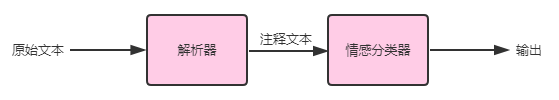
\includegraphics{./img/ch47_01.png}

最近的趋势更倾向于用一种单一的学习算法取代此类流水线。该任务的\textbf{端到端学习算法}只需输入一个原始的文本
``这个拖把非常好用!'' ,接着尝试直接识别其中的情感:

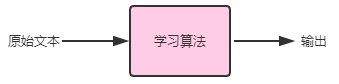
\includegraphics{./img/ch47_02.png}

神经网络通常用于端到端学习系统,``端到端''
这个术语指的是我们要求学习算法直接从输入得到期望的输出,即学习算法将系统的
``输入端'' 连接到 ``输出端'' 。

在数据量十分丰富的问题上,端到端系统往往很奏效,但它并不总是一个很好的选择。接下来的几个章节将给出更多的端到端系统的例子,并提供一些关于何时使用它们的建议。

\hypertarget{ux7aefux5230ux7aefux5b66ux4e60ux7684ux66f4ux591aux4f8bux5b50}{%
\chapter{端到端学习的更多例子}\label{ux7aefux5230ux7aefux5b66ux4e60ux7684ux66f4ux591aux4f8bux5b50}}

假设你正在构建一个语音识别系统,你的系统可能需要三个组件:

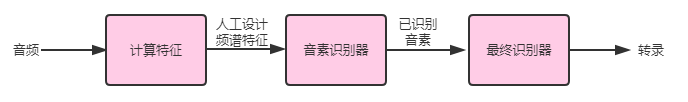
\includegraphics{./img/ch48_01.png}

它们的工作形式如下:

\begin{enumerate}
\def\labelenumi{\arabic{enumi}.}
\tightlist
\item
  计算特征(compute features):提取人工设计的特征,如 MFCC
  (Mel-frequency cepstrum
  coefficients,频谱系数)特征,以此来试图捕捉对话的内容,而忽略不太相关的属性,比如说话者的音高。
\item
  音素识别器(phoneme
  recognizer):一些语言学家人为,有一些基本的声音单元叫做 ``音素'' 。
  例如, ``keep'' 中的 ``k'' 和 ``cake'' 中的 ``c''
  是相同的音素,而这个系统试图识别音频片段中的音素。
\item
  最终识别器(final
  recognizer):以已识别音素的序列为序,并试着将它们串在一起,形成转录输出。
\end{enumerate}

与此相反,端到端系统可能会输入一个音频片段,并尝试直接输出文字记录:

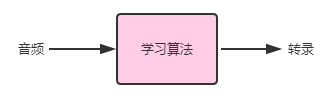
\includegraphics{./img/ch48_02.png}

到目前为止,我们只描述了纯线性的机器学习
``流水线'':输出顺序地从一个阶段传递到下一个阶段。实际上流水线可能会更复杂。例如,这是一个自动驾驶汽车的简单流水线架构:

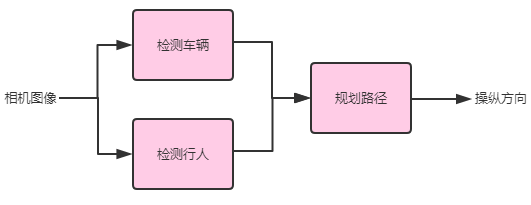
\includegraphics{./img/ch48_03.png}

它拥有三个组件:一个使用相机图片检测车辆,一个检测行人,最后一个组件则为我们自己的车规划路径,从而避让车辆和行人。

并不是流水线中的每一个组件都需要进行学习。例如在文献 ``robot motion
planning''
中对汽车的最终路径规划提出了许多算法,而其中的一些算法并不涉及到学习。

相反,端到端的方法可能会尝试从传感器获取输入并直接输出转向方向:

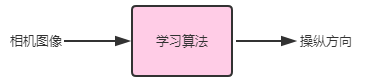
\includegraphics{./img/ch48_04.png}

尽管端到端学习已经在许多领域取得了成功,但它并不总是最佳方案。端到端的语音识别功能很不错,但我对自动驾驶的端到端学习持怀疑态度。在接下来的几章将会解释原因。

\hypertarget{ux7aefux5230ux7aefux5b66ux4e60ux7684ux4f18ux7f3aux70b9}{%
\chapter{端到端学习的优缺点}\label{ux7aefux5230ux7aefux5b66ux4e60ux7684ux4f18ux7f3aux70b9}}

考虑先前提到的语音识别系统的流水线:

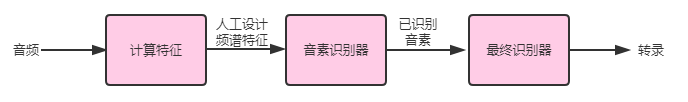
\includegraphics{./img/ch48_01.png}

该流水线中的许多部分都是 ``人工设计'' 的:

\begin{itemize}
\tightlist
\item
  频谱系数即是一套经过人工设计的特征。尽管它们提供了对音频输入的一种合理归纳,但也通过抛出一些信息简化了输入信号。
\item
  音素是语言学家的发明,作为说话声音的一种不完备的表示。在某种意义上,音素是对现实语音很差的近似,因此迫使算法使用音素进行表示将限制语音系统的性能。
\end{itemize}

这些人工设计的成分限制了语音系统的潜在性能,然而这样做也有一些优点:

\begin{itemize}
\tightlist
\item
  频谱系数的特性对于处理一些不影响内容的音频属性是很有效的,比如说话者的音高。因此它们有助于简化学习算法面临的问题。
\item
  在一定程度上,音素是一种合理的语音表示方法,它们也可以帮助学习算法理解基本的声音成分,从而提高其性能。
\end{itemize}

拥有更多的人工设计成分通常可以让语音系统学习更少的数据,由频谱系数和音素所捕获的人工设计的知识对算法从数据中获取的知识进行了补充。当我们的数据量不是很多时,这些知识是非常有用的。

现在,考虑端到端系统:

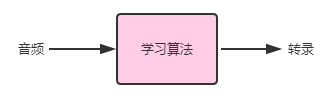
\includegraphics{./img/ch48_02.png}

这个系统缺乏人工设计知识,因此当训练集很小的时候,它的表现可能比人工设计的流水线更加糟糕。

然而当训练集很大时,它不会受到频谱系数或者语音表示方法的限制。如果学习算法是一个足够大的神经网络,且喂进去许多的训练数据,就有可能做得更好,甚至达到最优错误率。

端到端学习系统在 ``两端'' ------
输入端和输出端拥有大量标记数据时,往往做得更好。在这个例子中,我们需要一个大数据集(包含\textless 音频,文本\textgreater 对)。当这种类型的数据不可用时,使用端到端学习则需非常谨慎。

如果你正在研究一个训练集非常小的机器学习问题,那么算法的大部分知识都将来自于你的人类洞察力,即你的
``人工设计'' 成分。

如果不使用端到端系统,你将不得不决定在流水线中需要有哪些组件,以及它们应该如何连接在一起。在接下来的几章中,我们将对这类流水线的设计提出一些建议。

\hypertarget{ux6d41ux6c34ux7ebfux7ec4ux4ef6ux7684ux9009ux62e9ux6570ux636eux53efux7528ux6027}{%
\chapter{流水线组件的选择:数据可用性}\label{ux6d41ux6c34ux7ebfux7ec4ux4ef6ux7684ux9009ux62e9ux6570ux636eux53efux7528ux6027}}

在构建非端到端的流水线系统时,什么样的流水线组件可作为合适的选项呢?对流水线的设计将极大地影响整个系统的性能,其中一个重要因素是,是否能够轻松地收集到数据来训练每个组件。

例如,考虑下面这个自动驾驶架构:

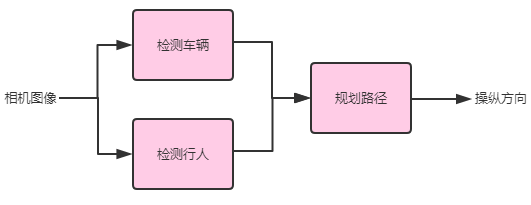
\includegraphics{./img/ch48_03.png}

你可以使用机器学习算法进行车辆和行人的检测,另外要获取这些数据也并非难事------如今有许多含有大量带车辆和行人标记的计算机视觉数据集。你也可以通过众包市场(比如
Amazon Mechanical
Turk)获得甚至更大规模的数据集。因此,获取训练数据来构建车辆检测器与行人检测器相对而言是比较容易的。

相反,考虑一种纯端到端的方式:

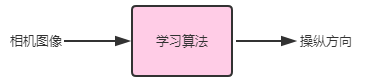
\includegraphics{./img/ch48_04.png}

为了训练这样一个系统,我们需要一个包含
\textless 图像,操纵方向\textgreater{}
数据对的大型数据集。然而让人们在驾驶汽车时收集汽车的操纵方向的数据是非常费时费力的,你需要一辆特殊配置的汽车,且需要巨大的驾驶量来涵盖各种可能的场景。这就使得端到端系统难以进行训练,获得大量带标记的行人或者是汽车图像反而要容易得多。

更常见的情况是,如果有大量的数据可以被用来训练流水线的 ``中间模块''
(例如汽车检测器或行人检测器),你便可以考虑使用多段的流水线架构。因为可以使用所有可用数据进行训练,所以这种结构可能是更优的。

在更多端到端数据变得可用之前,我相信非端到端的方法对于自动驾驶而言是更有希望的------它的体系架构更匹配于数据的可用性。

\hypertarget{ux6d41ux6c34ux7ebfux7ec4ux4ef6ux7684ux9009ux62e9ux4efbux52a1ux7b80ux5355ux6027}{%
\chapter{流水线组件的选择:任务简单性}\label{ux6d41ux6c34ux7ebfux7ec4ux4ef6ux7684ux9009ux62e9ux4efbux52a1ux7b80ux5355ux6027}}

除了数据可用性之外,你还应该考虑流水线组件选择的第二个因素:独立的组件使得任务简单了多少?你应该尽可能地选择那些易于构建或学习的独立流水线组件,但对一个组件而言,
``易于'' 学习指的是什么呢?

考虑下面列出的机器学习任务,它们的难度逐级递增:

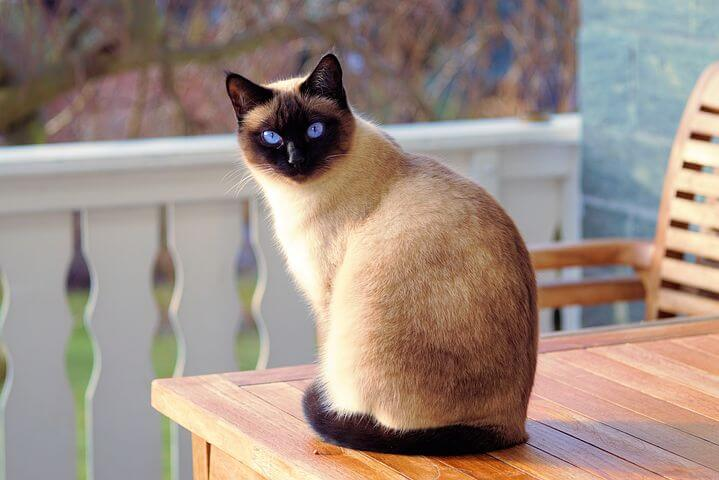
\includegraphics{./img/ch51_01.png}

\begin{enumerate}
\def\labelenumi{\arabic{enumi}.}
\tightlist
\item
  分类判断某张图片是否过度曝光(就像上面这张图片);
\item
  分类判断某张图片拍摄于室内还是室外;
\item
  分类判断某张图片中是否有猫;
\item
  分类判断某张图片中是否有黑白两色皮毛的猫;
\item
  分类判断某张图片中是否有暹罗猫(一种特殊的猫)
\end{enumerate}

这些图像分类任务都属于二分类任务------你需要输入一张图片,输出 0 或者 1.
但列出的前面几个任务看起来 ``更易于''
使神经网络进行学习。你将能够通过较少的训练样本来学习更加简单的任务。

对于使问题变得简单或困难的原因,机器学习领域尚未给出一个较好的正式定义。随着深度学习和多层神经网络的兴起,我们有时认为,如果一个任务可以用更少的计算步骤(对应于一个浅的神经网络)来实现,那么相对于需要更多的计算步骤(对应于一个深的神经网络),这个任务就
``更简单'' 了。但这些都是非正式的定义。

\begin{quote}
在信息论中有 ``Kolmogorov 复杂度''
的概念,一个学习函数的复杂度是产生该函数的计算机程序的最短长度。然而这一理论概念在人工智能领域几乎没有什么实际的应用。参考:https://en.wikipedia.org/wiki/Kolmogorov\_complexity
\end{quote}

如果你能够完成一个复杂的任务,并将其分解为更简单的子任务,然后显式编写子任务步骤代码,那么你就会给算法一些先验知识,从而帮助它更有效地学习任务。

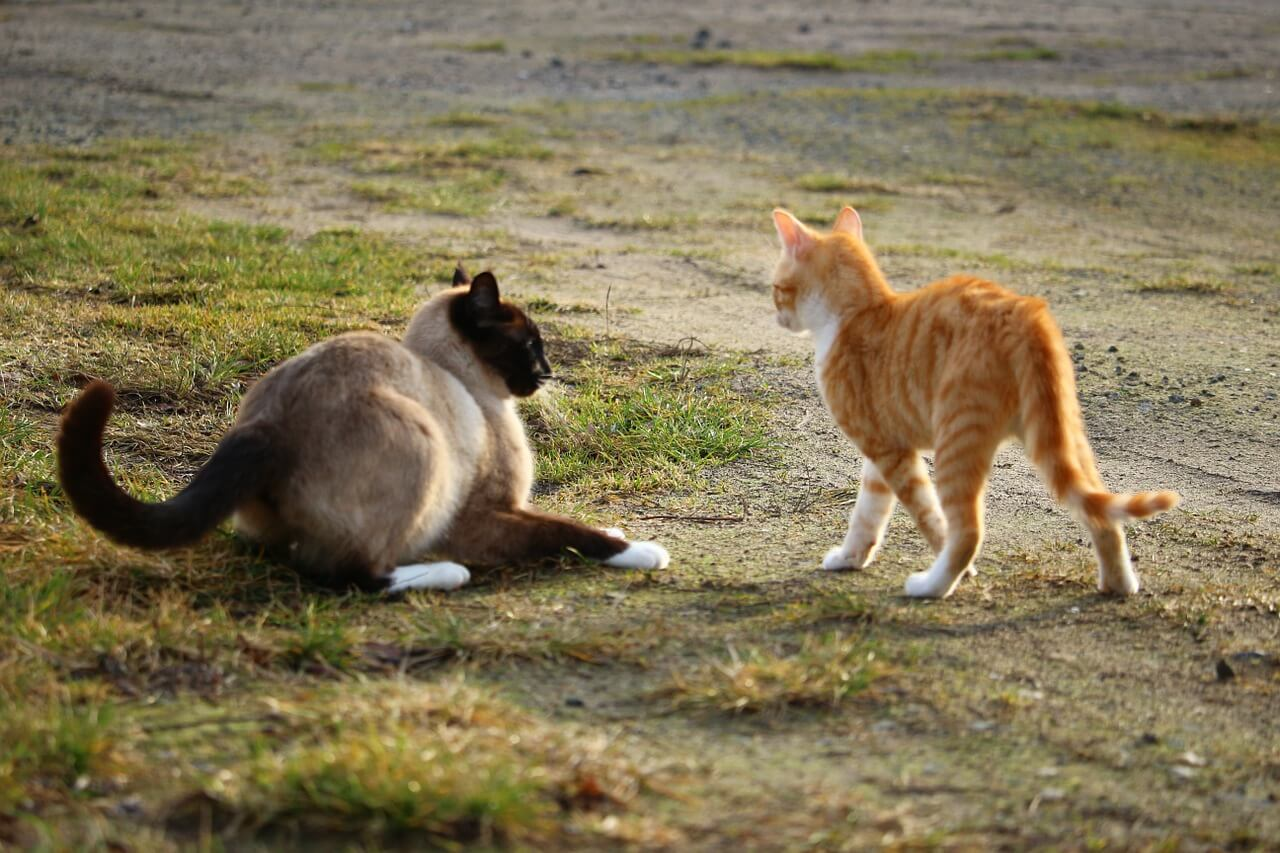
\includegraphics{./img/ch51_03.png}

假设你正在构建一个暹罗猫检测器。下面是一个纯粹的端到端架构:

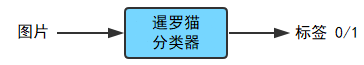
\includegraphics{./img/ch51_02.png}

与此相反,你可以分成两个步骤来形成流水线:

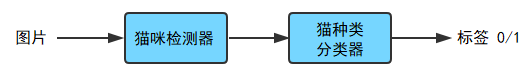
\includegraphics{./img/ch51_04.png}

第一步:(猫检测器)检测图像中所有的猫。

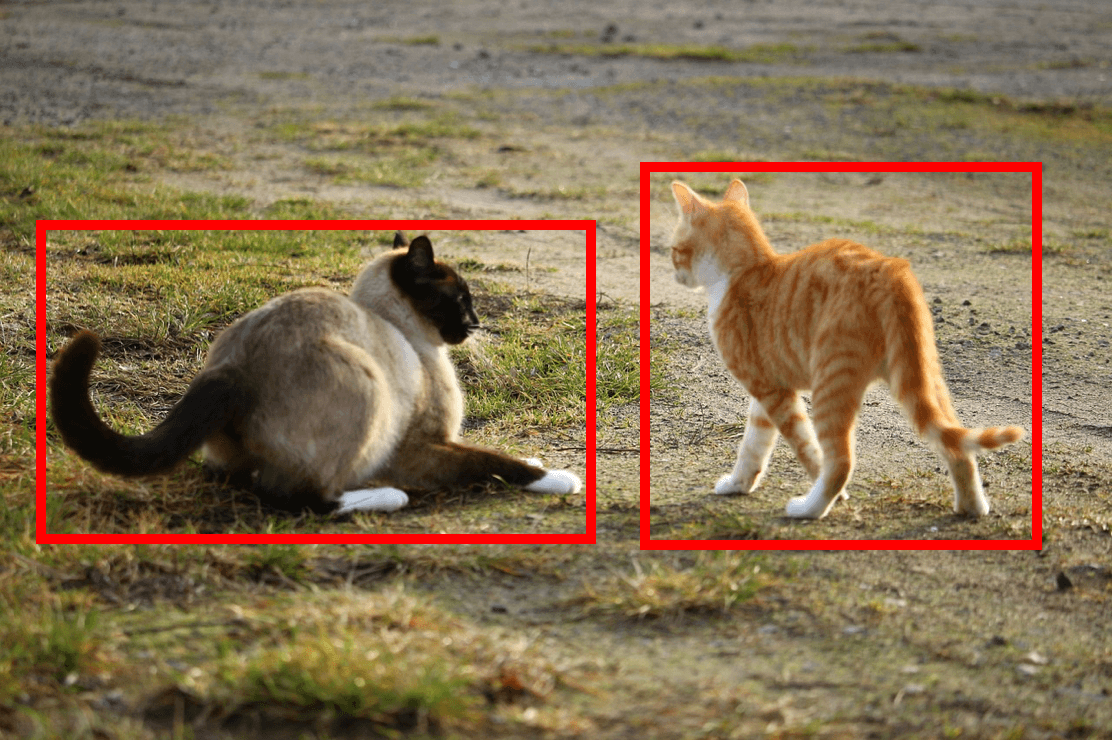
\includegraphics{./img/ch51_05.png}

第二步:将每一块被检测到的猫的图像传送给猫种类分类器(每次一张),如果其中任何一只猫是暹罗猫,则在最后输出
1.

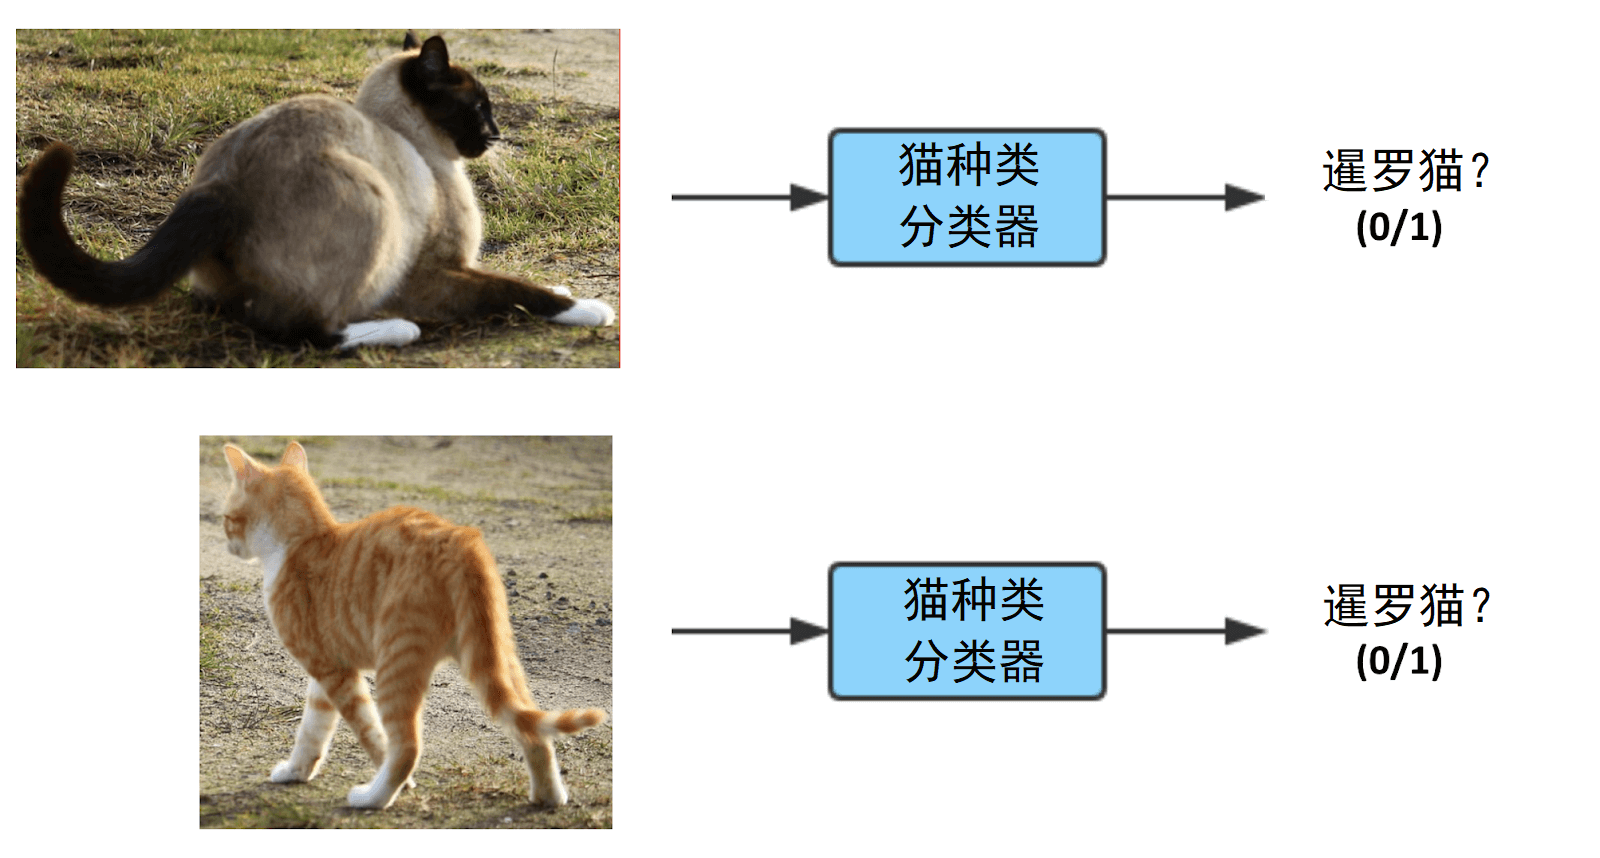
\includegraphics{./img/ch51_06.png}

与仅仅使用标签 0/1
来训练一个纯粹的端到端分类器相比,流水线中的两个组件------猫咪检测器和猫种类分类器------似乎更容易进行学习,而且需要更少的数据。

\begin{quote}
如果你熟悉实际运用中的对象检测算法,你将认识到它们并不是只学习 0/1
图像标签,而是作为训练数据的一部分取代边界框进行训练,对它们的讨论超出了本章的范围。如果你想了解更多关于这种算法的知识,请参阅
Coursera 的 Deep Learning 专项课程(http://deeplearning.ai)。
\end{quote}

最后一个例子,让我们回顾一下自动驾驶流水线。

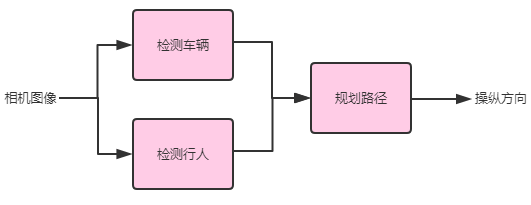
\includegraphics{./img/ch48_03.png}

通过使用该流水线架构,你可以告诉算法总共有三个关键的步骤:(1)检测其他车辆,(2)检测行人,(3)为你的车规划一条道路。此外,每一个步骤都是相对简单的功能------因此可以用更少的数据来学习------而不是纯粹的端到端方法。

总而言之,当决定流水线组件的内容组成时,试着构建这样的流水线,其中每个组件都是一个相对
``简单'' 的功能,因此只需要从少量的数据中学习。

\hypertarget{ux76f4ux63a5ux5b66ux4e60ux66f4ux4e3aux4e30ux5bccux7684ux8f93ux51fa}{%
\chapter{直接学习更为丰富的输出}\label{ux76f4ux63a5ux5b66ux4e60ux66f4ux4e3aux4e30ux5bccux7684ux8f93ux51fa}}

一个图像分类算法可以输入一个图像 \(x\)
,并输出一个表示对象类别的整数。那么一个算法可以输出一个完整的句子来对图像进行描述吗?

举个例子------

输入 \(x\) 为:

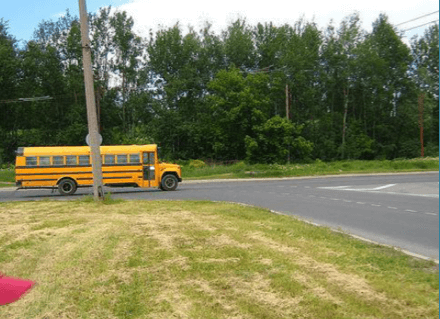
\includegraphics{./img/ch52_01.png}

输出 \(y\)
为:``一辆黄色的公共汽车在路上开着,背景是绿色的树和绿色的草。''

传统的监督学习应用学得一个函数:\(h:X \mapsto Y\) ,其中输出 \(Y\)
通常是一个整数或者实数。例如:

\begin{longtable}[]{@{}lll@{}}
\toprule
问题 & X & Y \\
\midrule
\endhead
垃圾邮件分类 & 邮件 & 垃圾邮件/非垃圾邮件 (0/1) \\
图像识别 & 图像 & 整数值标签 \\
房价预测 & 房屋特征 & 美元价格 \\
产品推荐 & 产品与用户特征 & 购买机率 \\
\bottomrule
\end{longtable}

端到端深度学习中最令人兴奋的进展之一是,它让我们直接学习比数字复杂得多的
\(y\) .
在上面的图像配字示例中,你可以使用一个神经网络输入一个图像(\(x\)),并直接输出一个标题(\(y\)).

下面有更多的例子:

\begin{longtable}[]{@{}llll@{}}
\toprule
问题 & X & Y & 文献引用 \\
\midrule
\endhead
图像配字 & 图像 & 文本 & Mao et al., 2014 \\
机器翻译 & 英语文本 & 法语文本 & Mao et al., 2014 \\
问题回答 & (文本,问题)对 & 回答文本 & Bordes et al., 2015 \\
语音识别 & 音频 & 转录 & Hannun et al., 2015 \\
文本转语音 & 文本特征 & 音频 & van der Oord et al., 2016 \\
\bottomrule
\end{longtable}

这体现了深度学习的高速变化趋势:当你有正确的(输入,输出)标签对的时候,有时可以进行端到端学习,即使输出是一个句子、图像、音频,或者其它的比一个数字更丰富的输出形式。

\hypertarget{ux6839ux636eux7ec4ux4ef6ux8fdbux884cux8befux5deeux5206ux6790}{%
\part{根据组件进行误差分析}\label{ux6839ux636eux7ec4ux4ef6ux8fdbux884cux8befux5deeux5206ux6790}}

\hypertarget{ux6839ux636eux7ec4ux4ef6ux8fdbux884cux8befux5deeux5206ux6790-1}{%
\chapter{根据组件进行误差分析}\label{ux6839ux636eux7ec4ux4ef6ux8fdbux884cux8befux5deeux5206ux6790-1}}

假设你的系统由复杂的机器学习流水线所构建,并且你希望提高该系统的性能,那应该从流水线的哪一部分开始改进呢?你可以通过将误差归因于流水线的特定组件,来决定工作的优先级。

我们使用暹罗猫分类器的例子来进行说明:

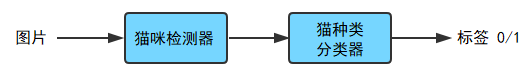
\includegraphics{./img/ch51_04.png}

在上图的流水线中,第一部分是猫检测器,它能够检测出猫,并将它们从图像裁剪出来;第二部分是猫的品种分类器,决定它是否是暹罗猫。
改进两个组件中的任何一个都有可能花费数年的时间。
你该决定关注哪个(些)组件呢?

通过\textbf{按组件进行误差分析},你可以尝试将每一个算法造成的误差归因于流水线的某个(有时是两个)组件。例如,即使某张图片样本的正确标签为含有暹罗猫(
\(y=1\)) ,算法依旧将其标签误分类为不含有暹罗猫(\(y=0\)).

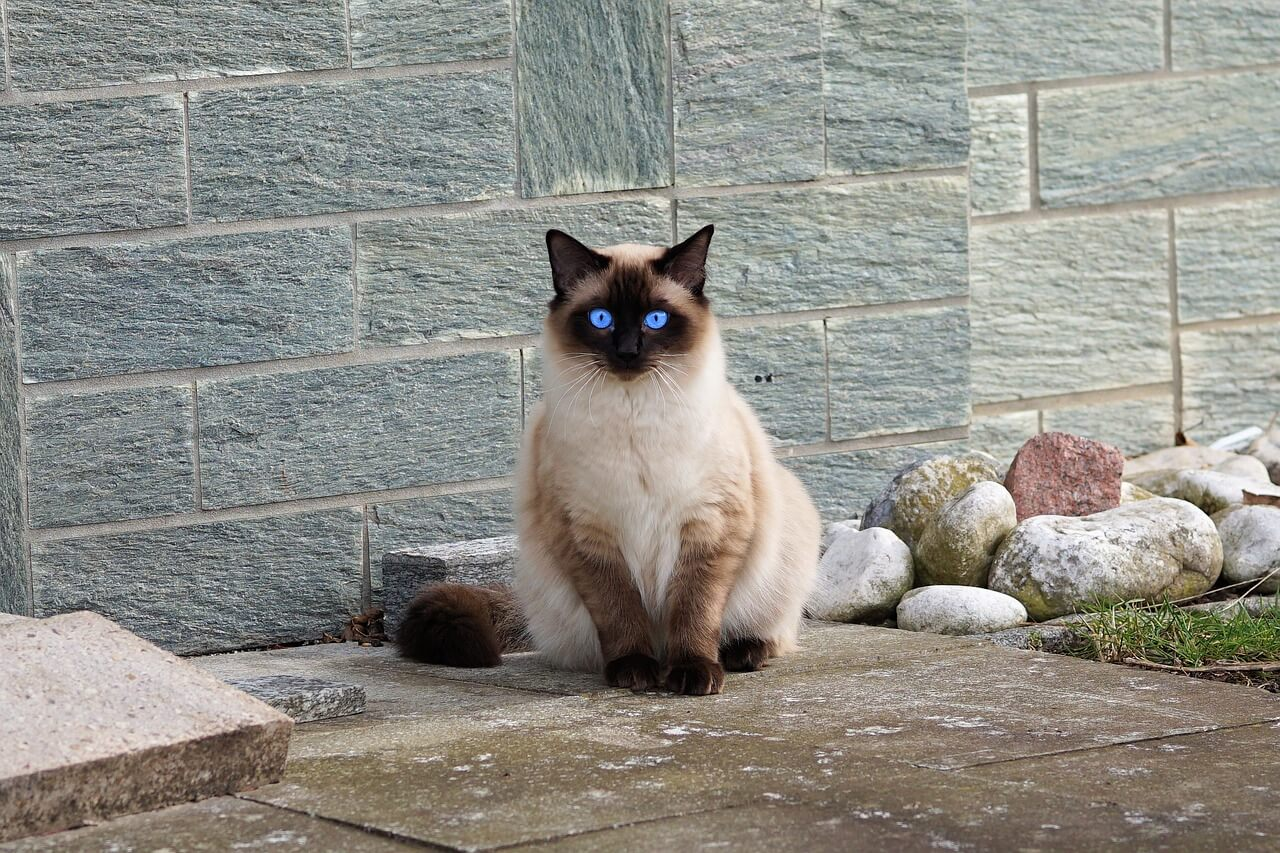
\includegraphics{./img/ch53_01.png}

让我们人为地检查一下算法两个步骤的执行过程。假设暹罗猫检测器从下图中检测出一只猫:

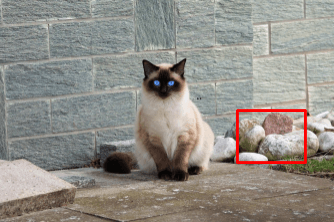
\includegraphics{./img/ch53_02.png}

这表示猫检测器给出了这样的图片:

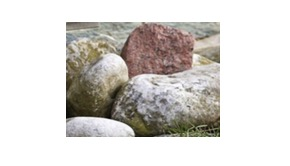
\includegraphics{./img/ch53_04.jpeg}

接下来,猫品种分类器将此图像正确分类为不包含暹罗猫。
因此,猫品种分类器是正常工作的:给它一堆岩石并输出一个非常合理的标签(\(y=0\)).
实际上,对上面裁剪的图像进行分类的人也会预测(\(y=0\)).
因此,你可以清楚地将此误差归因于猫探测器组件。
另一方面,如果猫探测器输出了以下边界框:

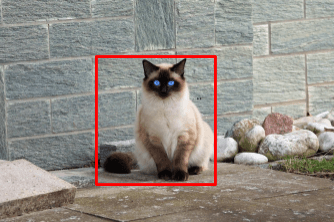
\includegraphics{./img/ch53_03.png}

你会得出如下结论,猫探测器已经完成了它的工作,并且它是有缺陷的猫品种分类器。

如果你对 100 个误分类的开发集图像遍历检查,并发现 90
个误差可归因于猫探测器,并只有 10 个误差可归因于猫品种分类器。
那么你可以有把握地得出结论,应该更加专注于改进猫探测器。

此外,你现在还可以方便地找到 90
个样本,其中猫探测器将输出不正确的边界框。 你可以使用这 90
个样本对猫探测器进行更深层次的误差分析,以了解该如何改进。

到目前为止,我们关于如何将误差归因于流水线的特定组件的描述是非正式的:查看每个组件的输出,并看看是否可以决定哪个部分出错了。
这种非正式的方法可能就是你所需要的。但在下一章中,你还将看到一种更正式的误差归因方式。

\hypertarget{ux8befux5deeux5f52ux56e0ux81f3ux67d0ux4e2aux7ec4ux4ef6}{%
\chapter{误差归因至某个组件}\label{ux8befux5deeux5f52ux56e0ux81f3ux67d0ux4e2aux7ec4ux4ef6}}

让我们继续使用这个例子:

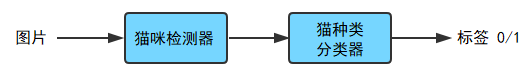
\includegraphics{./img/ch51_04.png}

假设猫检测器输出了这样的边界框:

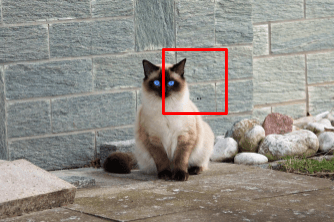
\includegraphics{./img/ch54_01.png}

被裁剪的图片将会送给猫品种分类器,因此它给出了错误的分类结果 \(y=0\) ,
即图片中没有猫。

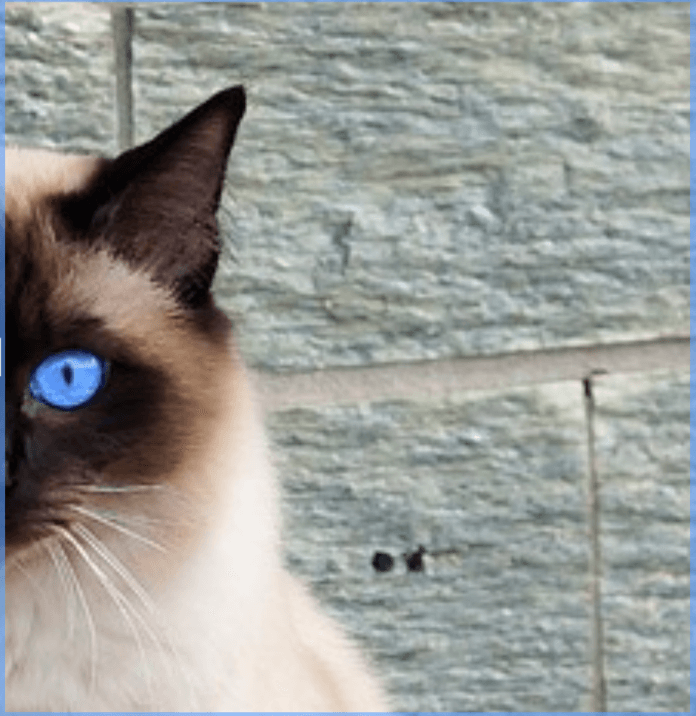
\includegraphics{./img/ch54_02.png}

猫检测器的效果很糟糕。
然而,一个技术娴熟的人类仍然可以从这种糟糕的裁剪图像中识别出暹罗猫。
那么我们是否可以将此误差归因于猫检测器或猫品种分类器两者之一(或两者兼有)呢?
答案是模棱两可的。

如果像这样模糊情况的数量很少,你可以做出你想要的任何决定并获得类似的结果。
但这里有一个更正式的测试方法,可以让你更明确地将误差归因于某一个组件:

\begin{enumerate}
\def\labelenumi{\arabic{enumi}.}
\tightlist
\item
  用手动标记的边界框替换猫检测器的输出。
\item
  通过猫品种分类器处理相应的裁剪图像。
  如果猫品种分类器仍将其错误地分类,则将误差归因于猫品种分类器。
  否则,将此误差归因于猫检测器。
\end{enumerate}

换而言之,进行一个实验,在其中为猫品种分类器提供 ``完美'' 输入。
有两种情况:

情况1:即使给出了一个 ``完美'' 的边界框,猫品种分类器仍然错误地输出
\(y = 0\). 在这种情况下,猫品种分类器很明显存在着问题。 情况2:给定一个
``完美'' 的边界框,品种分类器现在正确输出 \(y = 1\).
这表明只要猫检测器给出了一个更完美的边界框,那么整个系统的输出就是正确的。
因此,将误差归因于猫检测器。

通过对开发集误分类的图像执行此分析,你现在可以将每个误差明确地归因于一个组件。
这允许你对流水线不同组件所造成的误差程度进行估计,从而决定将注意力集中在哪儿。

\hypertarget{ux8befux5deeux5f52ux56e0ux7684ux4e00ux822cux60c5ux51b5}{%
\chapter{误差归因的一般情况}\label{ux8befux5deeux5f52ux56e0ux7684ux4e00ux822cux60c5ux51b5}}

以下是误差归因的一般步骤。 假设在流水线中有三个步骤 A,B 和 C,其中 A
直接输出到 B,B直接输出到 C.

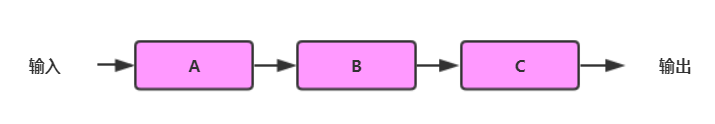
\includegraphics{./img/ch55_01.png}

对于系统在开发集上存在的每个错误样本:

\begin{enumerate}
\def\labelenumi{\arabic{enumi}.}
\tightlist
\item
  尝试人为修改 A 的输出为 ``完美'' 输出(例如,猫的 ``完美''
  边界框),并在此输出上运行流水线其余的 B,C 部分。
  如果算法现在给出了正确的输出,那么这表明,只要 A
  给出了更好的输出,那么整个算法的输出就是正确的;因此,你可以将此误差归因于组件
  A. 否则,请继续执行步骤 2.
\item
  尝试人为修改 B 的输出为 ``完美''
  输出。如果算法现在给出正确的输出,则将误差归因于组件 B.
  否则,继续执行步骤 3.
\item
  将误差归因于组件 C.
\end{enumerate}

让我们来看一个复杂一点的例子:

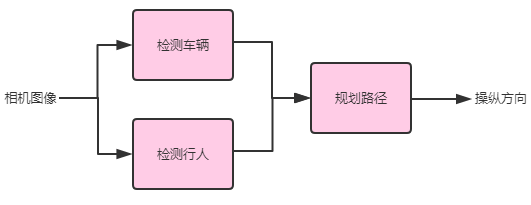
\includegraphics{./img/ch48_03.png}

你的自动驾驶汽车将使用上面的流水线技术。如何根据组件进行误差分析来决定专注于哪个(些)组件呢?

你可以将三个组件映射到 A, B, C,如下所示:

A:检测汽车 B:检测行人 C:规划汽车路径

按照上述程序,假设你在封闭的轨道上对你的汽车进行测试,发现汽车选择了一个比熟练司机更刺耳的转向方向。在自动驾驶领域,这种情况通常被称为\textbf{场景(scenario)}。接着你需要:

\begin{enumerate}
\def\labelenumi{\arabic{enumi}.}
\tightlist
\item
  尝试人为修改 A (检测汽车)的输出,使之成为 ``完美''
  输出(例如,手动进入并告诉它其他汽车在哪里)。像之前一样运行流水线其余的
  B,C 部分,但是允许 C (规划路径)使用 A
  现在的完美输出。如果算法现在为汽车规划出一条更好的路径,那么这表明,如果
  A 给出更好的输出,整个算法的输出会更好;因此,你可以将此误差归因于组件
  A. 否则,继续执行步骤 2.
\item
  尝试人为修改 B (检测行人)的输出,使之成为 ``完美''
  输出。如果算法现在给出了正确的输出,那么将误差归因为组件 B.
\item
  将误差归因于组件 C.
\end{enumerate}

ML
流水线的组件应该按照有向无环图(DAG)排序,这意味着你应该能够以某种固定的从左到右的顺序来计算它们,并且后面的组件应该只依赖于早期组件的输出。只要组件到
A-\textgreater B-\textgreater C 顺序的映射遵循 DAG
顺序,那么误差分析就没问题。但如果你交换 A 和
B,可能会得到略微不同的结果:

A:检测行人(以前是检测汽车)

B:检测汽车(以前是检测行人)

C:规划汽车路径

但是这个分析的结果仍然是有效的,并且可以很好地指导你把注意力集中在哪里。

\hypertarget{ux7ec4ux4ef6ux8befux5deeux5206ux6790ux4e0eux4ebaux7c7bux6c34ux5e73ux5bf9ux6bd4}{%
\chapter{组件误差分析与人类水平对比}\label{ux7ec4ux4ef6ux8befux5deeux5206ux6790ux4e0eux4ebaux7c7bux6c34ux5e73ux5bf9ux6bd4}}

对学习算法进行误差分析就像使用数据科学来分析 ML
系统的错误,以获得有关下一步该做什么的建议。从基本角度来看,组件误差分析告诉我们:哪些组件的性能是最值得尽力去改进的。

假设你有一个客户在网站上购物的数据集,数据科学家可能有许多不同的方法来分析数据。她可能会得出许多不同的结论------关于网站是否应该提高价格,关于通过不同营销活动获得的客户的终身价值等等。并不存在一种
``正确''
的方法来对数据集进行分析并得出许多可能有用的见解。同样,也没有一种
``正确''
的方法来进行误差分析。通过这些章节,你已经学习了许多最常见的设计模式,用于得到有关
ML 系统的有用见解,但你也可以自由尝试其他误差分析的方法。

让我们回到自动驾驶应用程序的讨论中,其中汽车检测算法输出附近汽车的位置(也可能是速度),行人检测算法输出附近行人的位置,这两个输出最终用于为当前车辆进行路径规划。

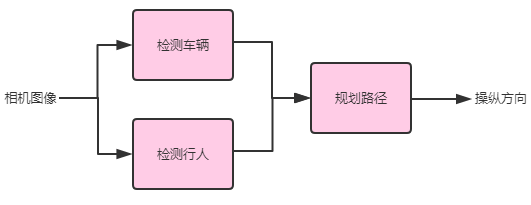
\includegraphics{./img/ch48_03.png}

如果想要调试该流水线,却不希望严格遵循上一章中提到的过程,你可以非正式地询问:

\begin{enumerate}
\def\labelenumi{\arabic{enumi}.}
\tightlist
\item
  在检测汽车时,汽车检测组件与人类水平表现相差多少?
\item
  在检测行人时,行人检测组件与人类水平表现相差多少?
\item
  整个系统的性能与人类表现相差多少?在这里,人类水平的表现假定:人类必须仅根据前两个流水线组件的输出(而不是访问摄像机图像)来规划汽车的路径。换句话说,当人类只得到相同的输入时,路径规划组件的性能与人类的性能相较如何?
\end{enumerate}

如果你发现其中一个组件远低于人类水平的表现,那么你现在可以专注于提高该组件的性能。

当我们尝试自动化人类可以做的事情时,许多误差分析过程将表现得最好,因此可以对人类水平的表现进行基准测试。
我们前面的大多数例子都有这个隐含的假设。 如果你正在构建
ML系统,其中最终输出或某些中间组件正在做甚至连人类都无法做好的事情,那么这些过程中的一些步骤将不起作用。

这是解决人类可解决的问题的另一个优势 -
你拥有更强大的误差分析工具,因此你可以更有效地优先处理团队的工作。

\hypertarget{ux53d1ux73b0ux6709ux7f3aux9677ux7684ux673aux5668ux5b66ux4e60ux6d41ux6c34ux7ebf}{%
\chapter{发现有缺陷的机器学习流水线}\label{ux53d1ux73b0ux6709ux7f3aux9677ux7684ux673aux5668ux5b66ux4e60ux6d41ux6c34ux7ebf}}

如果你的机器学习流水线的每个单独组件在人类水平性能或接近人类水平性能上执行,但总体流水线性能却远远低于人类水平会怎么样?这通常意味着流水线存在缺陷,需要重新设计。
误差分析还可以帮助你了解是否需要重新设计流水线。

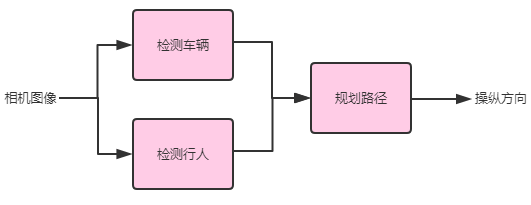
\includegraphics{./img/ch48_03.png}

在前一章中,我们提出了这三个部分组件的表现是否达到人类水平的问题。假设所有三个问题的答案都是肯定的,也即是说:

\begin{enumerate}
\def\labelenumi{\arabic{enumi}.}
\tightlist
\item
  汽车检测部件(大概)是人类级别的性能,用于从摄像机图像中检测汽车。
\item
  行人检测组件(大概)是人类级别的性能,用于从摄像机图像中检测行人。
\item
  与仅根据前两个流水线组件的输出(而不是访问摄像机图像)规划汽车路径的人相比,路径规划组件的性能处于类似水平。
\end{enumerate}

然而,你的自动驾驶汽车的整体性能远远低于人类水平。即,能够访问摄像机图像的人可以为汽车规划出明显更好的路径。据此你能得出什么结论?

唯一可能的结论是, ML
流水线存在着缺陷。在这种情况下,路径规划组件在给定输出的情况下可以做得很好,但输入没能包含足够的信息。你应该询问自己,除了两个早期流水线组件的输出之外,还需要哪些其他信息来为汽车的驾驶辅助规划路径。换句话说,熟练的人类驾驶员还需要什么其他信息?

例如,假设你意识到人类驾驶员还需要知道车道标记的位置。
这表明你应该按如下方式重新设计流水线:

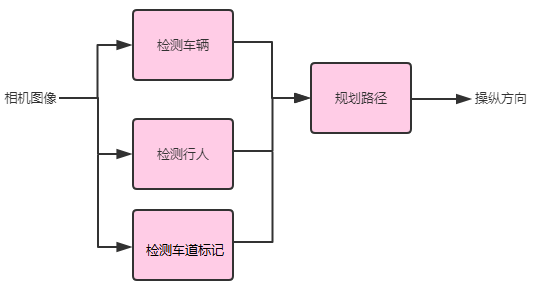
\includegraphics{./img/ch57_01.png}

最后,如果你认为,即使每个组件都具有人类级别的性能(请记住,你要与被给予与组件相同输入的人类进行比较),流水线整体上也不会达到人类水平的性能,则表明流水线有缺陷,应该重新设计。

\begin{quote}
在上面的自动驾驶案例中,理论上可以通过将原始相机图像馈送到路径规划组件中来解决该问题。
但是,这违反了第51章中描述的 ``任务简单性''
的设计原则,因为路径规划模块现在需要输入原始图像并且需要解决非常复杂的任务。
这就是添加车道标记检测组件是更好选择的原因 ------
它有助于将重要的和以前缺少的有关车道标记的信息提供给路径规划模块,但可以避免使任何过于复杂而无法构建/训练的特定模块。
\end{quote}

\hypertarget{ux603bux7ed3}{%
\part{总结}\label{ux603bux7ed3}}

\hypertarget{ux5efaux7acbux8d85ux7ea7ux82f1ux96c4ux56e2ux961f---ux8ba9ux4f60ux7684ux961fux53cbux9605ux8bfbux8fd9ux672cux4e66ux5427}{%
\chapter{建立超级英雄团队 -
让你的队友阅读这本书吧!}\label{ux5efaux7acbux8d85ux7ea7ux82f1ux96c4ux56e2ux961f---ux8ba9ux4f60ux7684ux961fux53cbux9605ux8bfbux8fd9ux672cux4e66ux5427}}

恭喜你完成这本书的阅读!

在第2章中,我们讨论了本书如何帮助你成为团队的超级英雄。

唯一比成为超级英雄更好的事情就是成为超级英雄团队的一员。
我希望你能把这本书的副本交给你的朋友和队友,并帮助创造出其他的超级英雄!
